% Options for packages loaded elsewhere
\PassOptionsToPackage{unicode}{hyperref}
\PassOptionsToPackage{hyphens}{url}
\PassOptionsToPackage{dvipsnames,svgnames,x11names}{xcolor}
%
\documentclass[
  letterpaper,
  DIV=11,
  numbers=noendperiod]{scrartcl}

\usepackage{amsmath,amssymb}
\usepackage{iftex}
\ifPDFTeX
  \usepackage[T1]{fontenc}
  \usepackage[utf8]{inputenc}
  \usepackage{textcomp} % provide euro and other symbols
\else % if luatex or xetex
  \usepackage{unicode-math}
  \defaultfontfeatures{Scale=MatchLowercase}
  \defaultfontfeatures[\rmfamily]{Ligatures=TeX,Scale=1}
\fi
\usepackage{lmodern}
\ifPDFTeX\else  
    % xetex/luatex font selection
\fi
% Use upquote if available, for straight quotes in verbatim environments
\IfFileExists{upquote.sty}{\usepackage{upquote}}{}
\IfFileExists{microtype.sty}{% use microtype if available
  \usepackage[]{microtype}
  \UseMicrotypeSet[protrusion]{basicmath} % disable protrusion for tt fonts
}{}
\makeatletter
\@ifundefined{KOMAClassName}{% if non-KOMA class
  \IfFileExists{parskip.sty}{%
    \usepackage{parskip}
  }{% else
    \setlength{\parindent}{0pt}
    \setlength{\parskip}{6pt plus 2pt minus 1pt}}
}{% if KOMA class
  \KOMAoptions{parskip=half}}
\makeatother
\usepackage{xcolor}
\setlength{\emergencystretch}{3em} % prevent overfull lines
\setcounter{secnumdepth}{5}
% Make \paragraph and \subparagraph free-standing
\ifx\paragraph\undefined\else
  \let\oldparagraph\paragraph
  \renewcommand{\paragraph}[1]{\oldparagraph{#1}\mbox{}}
\fi
\ifx\subparagraph\undefined\else
  \let\oldsubparagraph\subparagraph
  \renewcommand{\subparagraph}[1]{\oldsubparagraph{#1}\mbox{}}
\fi

\usepackage{color}
\usepackage{fancyvrb}
\newcommand{\VerbBar}{|}
\newcommand{\VERB}{\Verb[commandchars=\\\{\}]}
\DefineVerbatimEnvironment{Highlighting}{Verbatim}{commandchars=\\\{\}}
% Add ',fontsize=\small' for more characters per line
\usepackage{framed}
\definecolor{shadecolor}{RGB}{241,243,245}
\newenvironment{Shaded}{\begin{snugshade}}{\end{snugshade}}
\newcommand{\AlertTok}[1]{\textcolor[rgb]{0.68,0.00,0.00}{#1}}
\newcommand{\AnnotationTok}[1]{\textcolor[rgb]{0.37,0.37,0.37}{#1}}
\newcommand{\AttributeTok}[1]{\textcolor[rgb]{0.40,0.45,0.13}{#1}}
\newcommand{\BaseNTok}[1]{\textcolor[rgb]{0.68,0.00,0.00}{#1}}
\newcommand{\BuiltInTok}[1]{\textcolor[rgb]{0.00,0.23,0.31}{#1}}
\newcommand{\CharTok}[1]{\textcolor[rgb]{0.13,0.47,0.30}{#1}}
\newcommand{\CommentTok}[1]{\textcolor[rgb]{0.37,0.37,0.37}{#1}}
\newcommand{\CommentVarTok}[1]{\textcolor[rgb]{0.37,0.37,0.37}{\textit{#1}}}
\newcommand{\ConstantTok}[1]{\textcolor[rgb]{0.56,0.35,0.01}{#1}}
\newcommand{\ControlFlowTok}[1]{\textcolor[rgb]{0.00,0.23,0.31}{#1}}
\newcommand{\DataTypeTok}[1]{\textcolor[rgb]{0.68,0.00,0.00}{#1}}
\newcommand{\DecValTok}[1]{\textcolor[rgb]{0.68,0.00,0.00}{#1}}
\newcommand{\DocumentationTok}[1]{\textcolor[rgb]{0.37,0.37,0.37}{\textit{#1}}}
\newcommand{\ErrorTok}[1]{\textcolor[rgb]{0.68,0.00,0.00}{#1}}
\newcommand{\ExtensionTok}[1]{\textcolor[rgb]{0.00,0.23,0.31}{#1}}
\newcommand{\FloatTok}[1]{\textcolor[rgb]{0.68,0.00,0.00}{#1}}
\newcommand{\FunctionTok}[1]{\textcolor[rgb]{0.28,0.35,0.67}{#1}}
\newcommand{\ImportTok}[1]{\textcolor[rgb]{0.00,0.46,0.62}{#1}}
\newcommand{\InformationTok}[1]{\textcolor[rgb]{0.37,0.37,0.37}{#1}}
\newcommand{\KeywordTok}[1]{\textcolor[rgb]{0.00,0.23,0.31}{#1}}
\newcommand{\NormalTok}[1]{\textcolor[rgb]{0.00,0.23,0.31}{#1}}
\newcommand{\OperatorTok}[1]{\textcolor[rgb]{0.37,0.37,0.37}{#1}}
\newcommand{\OtherTok}[1]{\textcolor[rgb]{0.00,0.23,0.31}{#1}}
\newcommand{\PreprocessorTok}[1]{\textcolor[rgb]{0.68,0.00,0.00}{#1}}
\newcommand{\RegionMarkerTok}[1]{\textcolor[rgb]{0.00,0.23,0.31}{#1}}
\newcommand{\SpecialCharTok}[1]{\textcolor[rgb]{0.37,0.37,0.37}{#1}}
\newcommand{\SpecialStringTok}[1]{\textcolor[rgb]{0.13,0.47,0.30}{#1}}
\newcommand{\StringTok}[1]{\textcolor[rgb]{0.13,0.47,0.30}{#1}}
\newcommand{\VariableTok}[1]{\textcolor[rgb]{0.07,0.07,0.07}{#1}}
\newcommand{\VerbatimStringTok}[1]{\textcolor[rgb]{0.13,0.47,0.30}{#1}}
\newcommand{\WarningTok}[1]{\textcolor[rgb]{0.37,0.37,0.37}{\textit{#1}}}

\providecommand{\tightlist}{%
  \setlength{\itemsep}{0pt}\setlength{\parskip}{0pt}}\usepackage{longtable,booktabs,array}
\usepackage{calc} % for calculating minipage widths
% Correct order of tables after \paragraph or \subparagraph
\usepackage{etoolbox}
\makeatletter
\patchcmd\longtable{\par}{\if@noskipsec\mbox{}\fi\par}{}{}
\makeatother
% Allow footnotes in longtable head/foot
\IfFileExists{footnotehyper.sty}{\usepackage{footnotehyper}}{\usepackage{footnote}}
\makesavenoteenv{longtable}
\usepackage{graphicx}
\makeatletter
\def\maxwidth{\ifdim\Gin@nat@width>\linewidth\linewidth\else\Gin@nat@width\fi}
\def\maxheight{\ifdim\Gin@nat@height>\textheight\textheight\else\Gin@nat@height\fi}
\makeatother
% Scale images if necessary, so that they will not overflow the page
% margins by default, and it is still possible to overwrite the defaults
% using explicit options in \includegraphics[width, height, ...]{}
\setkeys{Gin}{width=\maxwidth,height=\maxheight,keepaspectratio}
% Set default figure placement to htbp
\makeatletter
\def\fps@figure{htbp}
\makeatother
% definitions for citeproc citations
\NewDocumentCommand\citeproctext{}{}
\NewDocumentCommand\citeproc{mm}{%
  \begingroup\def\citeproctext{#2}\cite{#1}\endgroup}
\makeatletter
 % allow citations to break across lines
 \let\@cite@ofmt\@firstofone
 % avoid brackets around text for \cite:
 \def\@biblabel#1{}
 \def\@cite#1#2{{#1\if@tempswa , #2\fi}}
\makeatother
\newlength{\cslhangindent}
\setlength{\cslhangindent}{1.5em}
\newlength{\csllabelwidth}
\setlength{\csllabelwidth}{3em}
\newenvironment{CSLReferences}[2] % #1 hanging-indent, #2 entry-spacing
 {\begin{list}{}{%
  \setlength{\itemindent}{0pt}
  \setlength{\leftmargin}{0pt}
  \setlength{\parsep}{0pt}
  % turn on hanging indent if param 1 is 1
  \ifodd #1
   \setlength{\leftmargin}{\cslhangindent}
   \setlength{\itemindent}{-1\cslhangindent}
  \fi
  % set entry spacing
  \setlength{\itemsep}{#2\baselineskip}}}
 {\end{list}}
\usepackage{calc}
\newcommand{\CSLBlock}[1]{\hfill\break\parbox[t]{\linewidth}{\strut\ignorespaces#1\strut}}
\newcommand{\CSLLeftMargin}[1]{\parbox[t]{\csllabelwidth}{\strut#1\strut}}
\newcommand{\CSLRightInline}[1]{\parbox[t]{\linewidth - \csllabelwidth}{\strut#1\strut}}
\newcommand{\CSLIndent}[1]{\hspace{\cslhangindent}#1}

\usepackage{booktabs}
\usepackage{caption}
\usepackage{longtable}
\usepackage{colortbl}
\usepackage{array}
\KOMAoption{captions}{tableheading}
\makeatletter
\@ifpackageloaded{caption}{}{\usepackage{caption}}
\AtBeginDocument{%
\ifdefined\contentsname
  \renewcommand*\contentsname{Table of contents}
\else
  \newcommand\contentsname{Table of contents}
\fi
\ifdefined\listfigurename
  \renewcommand*\listfigurename{List of Figures}
\else
  \newcommand\listfigurename{List of Figures}
\fi
\ifdefined\listtablename
  \renewcommand*\listtablename{List of Tables}
\else
  \newcommand\listtablename{List of Tables}
\fi
\ifdefined\figurename
  \renewcommand*\figurename{Figure}
\else
  \newcommand\figurename{Figure}
\fi
\ifdefined\tablename
  \renewcommand*\tablename{Table}
\else
  \newcommand\tablename{Table}
\fi
}
\@ifpackageloaded{float}{}{\usepackage{float}}
\floatstyle{ruled}
\@ifundefined{c@chapter}{\newfloat{codelisting}{h}{lop}}{\newfloat{codelisting}{h}{lop}[chapter]}
\floatname{codelisting}{Listing}
\newcommand*\listoflistings{\listof{codelisting}{List of Listings}}
\makeatother
\makeatletter
\makeatother
\makeatletter
\@ifpackageloaded{caption}{}{\usepackage{caption}}
\@ifpackageloaded{subcaption}{}{\usepackage{subcaption}}
\makeatother
\ifLuaTeX
  \usepackage{selnolig}  % disable illegal ligatures
\fi
\usepackage{bookmark}

\IfFileExists{xurl.sty}{\usepackage{xurl}}{} % add URL line breaks if available
\urlstyle{same} % disable monospaced font for URLs
\hypersetup{
  pdftitle={Comparative Analysis of Machine Learning Models for Thyroid Cancer Recurrence Prediction},
  pdfauthor={Anay Aggarwal; Ekam Kaur; Susie Lu},
  pdfkeywords={Cancer Research, Machine
Learning, ANN, KNN, SVM, Logistic Regression, XGBoost, Random Forest},
  colorlinks=true,
  linkcolor={blue},
  filecolor={Maroon},
  citecolor={Blue},
  urlcolor={Blue},
  pdfcreator={LaTeX via pandoc}}

\title{Comparative Analysis of Machine Learning Models for Thyroid
Cancer Recurrence Prediction}
\author{Anay Aggarwal \and Ekam Kaur \and Susie Lu}
\date{2024-06-15}

\begin{document}
\maketitle
\begin{abstract}
This study assesses the efficacy of machine learning
algorithms---Artificial Neural Network, K-Nearest Neighbors, Support
Vector Machine, Logistic Regression, Extreme Gradient Boosting, and
Random Forest---in predicting recurrence in Differentiated Thyroid
Cancer (DTC). Using a comprehensive dataset from the UCI Machine
Learning Repository, we conduct a comparative analysis of these
algorithms based on key performance metrics. Our investigation seeks to
identify the optimal model for enhancing DTC recurrence predictions,
aiming to advance personalized treatment strategies and improve clinical
outcomes in thyroid cancer care.
\end{abstract}

\section{Introduction}\label{introduction}

Thyroid cancer is among the most prevalent endocrine malignancies
worldwide, with differentiated thyroid cancer (DTC) representing the
majority of cases {[}1{]}. The management and prognosis of thyroid
cancer critically depend on the timely and accurate prediction of cancer
recurrence. Traditional approaches, primarily based on clinical and
pathological parameters, often lack the precision required for
personalized treatment planning {[}2{]}. With advancements in machine
learning (ML) techniques, there's a burgeoning interest in leveraging
these analytical tools to enhance the predictive accuracy regarding
cancer recurrence, thereby improving the efficacy of therapeutic
interventions and follow-up strategies {[}3{]}.

This paper explores the application of six distinct machine learning
algorithms---Artificial Neural Network (ANN), Support Vector Machine
(SVM), K-Nearest Neighbors (KNN), Logistic Regression (LR), and the
ensemble learning methods -- Random Forest (RF) and Extreme Gradient
Boosting (XGBoost) --- to predict cancer recurrence in patients with
differentiated thyroid cancer. Utilizing the differentiated thyroid
cancer recurrence dataset from the UCI Machine Learning Repository
{[}4{]}, this study aims to compare the predictive performance of these
algorithms in a clinical setting. The dataset comprises patient
demographic information, clinical features, and pathological details,
providing a solid foundation for predictive modeling.

ANNs, celebrated for their capability to model complex nonlinear
relationships through interconnected processing elements, offer powerful
tools for medical prediction tasks {[}5{]}. SVMs, recognized for their
effectiveness in high-dimensional spaces and versatility in handling
both linear and nonlinear data, present a robust methodology for
classification challenges {[}6{]}. KNN, a straightforward yet efficient
algorithm based on feature space proximity, offers an intuitive approach
to classification by leveraging the similarity between cases {[}7{]}.
LR, known for its simplicity and efficient training, offers a intuitive
way for determining the decision boundary between linearly separable
data points, and directly outputs the predicted probabilities for each
class {[}8{]}. RF, an ensemble learning method that uses bagging on
classification trees, proves to be efficient and accurate in handling
high-dimensional and non-linear data {[}9{]}. XGBoost, an ensemble
learning method that uses boosting (meaning that the algorithm
sequentially generates new trees based on previous training output), is
very fast and robust for a variety of tasks {[}10{]}.

By applying all six machine learning approaches to the differentiated
thyroid cancer recurrence dataset, this study seeks to identify the most
effective model for predicting cancer recurrence, thus contributing to
the ongoing efforts to enhance patient outcomes in thyroid cancer
management.

Through a rigorous evaluation of model performance based on accuracy,
precision, recall, and specificity, this paper aims to shed light on the
strengths and limitations of each algorithm in the context of thyroid
cancer recurrence prediction. Furthermore, the study discusses the
implications of these findings for clinical practice, emphasizing the
potential of machine learning to revolutionize cancer care by enabling
more accurate and personalized risk assessments {[}11{]}

\section{Notation}\label{notation}

Suppose we have a quantitative response \(Y\) and \(p\) different
predictors \(X_1, X_2, \dots, X_p\). We assume that there is some
relationship between \(Y\) and \(X = (X_1, X_2, \dots, X_p)\), which can
be written in the general form \[Y = f(X) + \epsilon.\] Here \(f\) is
some fixed but unknown function of \(X_1, X_2, \dots, X_p\) and
\(\epsilon\) is a random error term, which is independent of \(X\) and
has mean zero. Our models will not be concerned with the form of \(f\)
but rather will try to formulate an estimate \(\hat{f}\) of \(f\) that
in turn produces an estimate \(\hat{Y}\) of \(Y\). The formulation of
interest becomes \[\hat{Y} = \hat{f}(X),\] where \(\hat{f}\) is treated
as a black box and the mean-zero error \(\epsilon\) is dropped.

Suppose the outcome is the set with classes \(1, 2, \dots, n\). The
Bayes Classifier assigns each observation to the most likely class,
given its predictor values. In other words, we assign class
\(j \in \{1, 2, \dots, n\}\) to the test observation \(x_0\) if
\[Pr(Y = j | X = x_0) = \max_{i} Pr(Y = i | X = x_0)\]

The Bayes classifier produces the lowest possible test error rate called
the Bayes error rate. In other words, the Bayes classifier minimizes the
test error defined by
\[\frac{1}{2} \sum_{i = 1}^{n} I(y_i \neq \hat{y}_i),\]

where \(I(y_i \neq \hat{y}_i)\) is an indicator variable that equals
\(1\) if \(y_i \neq \hat{y}_i\) and zero if \(y_i = \hat{y}_i\) (i.e.,
the \(i\)th observation was classified correctly). The Bayes decision
boundary is determines by those observations which conditional
probability is exactly \(0.5\).

\section{Data Analysis}\label{data-analysis}

Our study focuses on the ``Differentiated Thyroid Cancer Recurrence''
dataset {[}4{]} hosted by the UCI Machine Learning Repository. The UCI
Machine Learning Repository offers a wide array of datasets used for
empirical analysis in machine learning and data mining {[}12{]}.
Established by the University of California, Irvine, this repository
facilitates academic and educational pursuits by providing free access
to datasets that cover various domains. As of March, 2024, it hosts and
maintains over 600 datasets.

The ``Differentiated Thyroid Cancer Recurrence'' dataset encompasses 383
samples or observations, and a range of 17 variables pertinent to
thyroid cancer, including patient demographics, clinical features, and
pathological details, all aimed at elucidating patterns associated with
cancer recurrence.

We will employ six distinct modeling methods to analyze our dataset:
Artificial Neural Network (ANN), K-Nearest Neighbors (KNN), Support
Vector Machine (SVM), Logistic Regression (LR), Random Forest (RF), and
Extreme Gradient Boosting (XGBoost). Each of these methods brings unique
strengths to the analysis, with ANN providing deep learning
capabilities, KNN offering simplicity and ease of interpretation, SVM
delivering powerful discriminative classification, LR providing an
intuitive and easily trainable implementation, and the ensemble methods
RF and XGBoost offering highly robust and accurate tree algorithms --
thereby encompassing a comprehensive approach to predicting cancer
recurrence in the studied dataset.

To prepare our data for modeling, we fix a typo, remove duplicate
observations, and transform the categorical variables into factors.

\begin{Shaded}
\begin{Highlighting}[]
\CommentTok{\#\textquotesingle{} Load raw data.}
\NormalTok{cleaned\_data }\OtherTok{\textless{}{-}} 
\NormalTok{  readr}\SpecialCharTok{::}\FunctionTok{read\_csv}\NormalTok{(here}\SpecialCharTok{::}\FunctionTok{here}\NormalTok{(}\StringTok{\textquotesingle{}data/raw{-}data.csv\textquotesingle{}}\NormalTok{)) }\SpecialCharTok{|\textgreater{}}
  \CommentTok{\# Remove duplicates.}
\NormalTok{  dplyr}\SpecialCharTok{::}\FunctionTok{distinct}\NormalTok{() }\SpecialCharTok{|\textgreater{}}
  \CommentTok{\# Fix column name typo.}
\NormalTok{  dplyr}\SpecialCharTok{::}\FunctionTok{rename}\NormalTok{(}\StringTok{\textasciigrave{}}\AttributeTok{Hx Radiotherapy}\StringTok{\textasciigrave{}} \OtherTok{=} \StringTok{\textquotesingle{}Hx Radiothreapy\textquotesingle{}}\NormalTok{) }\SpecialCharTok{|\textgreater{}}
\NormalTok{  dplyr}\SpecialCharTok{::}\FunctionTok{mutate}\NormalTok{(}\AttributeTok{Gender =} \FunctionTok{ifelse}\NormalTok{(Gender }\SpecialCharTok{==} \StringTok{\textquotesingle{}F\textquotesingle{}}\NormalTok{, }\StringTok{\textquotesingle{}Female\textquotesingle{}}\NormalTok{, }\StringTok{\textquotesingle{}Male\textquotesingle{}}\NormalTok{)) }\SpecialCharTok{|\textgreater{}}
\NormalTok{  dplyr}\SpecialCharTok{::}\FunctionTok{mutate}\NormalTok{(}
    \AttributeTok{Gender =} \FunctionTok{factor}\NormalTok{(Gender, }\AttributeTok{levels =} \FunctionTok{c}\NormalTok{(}\StringTok{\textquotesingle{}Female\textquotesingle{}}\NormalTok{, }\StringTok{\textquotesingle{}Male\textquotesingle{}}\NormalTok{)),}
    \AttributeTok{Smoking =} \FunctionTok{factor}\NormalTok{(Smoking, }\AttributeTok{levels =} \FunctionTok{c}\NormalTok{(}\StringTok{\textquotesingle{}Yes\textquotesingle{}}\NormalTok{, }\StringTok{\textquotesingle{}No\textquotesingle{}}\NormalTok{)),}
    \StringTok{\textasciigrave{}}\AttributeTok{Hx Smoking}\StringTok{\textasciigrave{}} \OtherTok{=} \FunctionTok{factor}\NormalTok{(}\StringTok{\textasciigrave{}}\AttributeTok{Hx Smoking}\StringTok{\textasciigrave{}}\NormalTok{, }\AttributeTok{levels =} \FunctionTok{c}\NormalTok{(}\StringTok{\textquotesingle{}Yes\textquotesingle{}}\NormalTok{, }\StringTok{\textquotesingle{}No\textquotesingle{}}\NormalTok{)),}
    \StringTok{\textasciigrave{}}\AttributeTok{Hx Radiotherapy}\StringTok{\textasciigrave{}} \OtherTok{=} \FunctionTok{factor}\NormalTok{(}\StringTok{\textasciigrave{}}\AttributeTok{Hx Radiotherapy}\StringTok{\textasciigrave{}}\NormalTok{, }\AttributeTok{levels =} \FunctionTok{c}\NormalTok{(}\StringTok{\textquotesingle{}Yes\textquotesingle{}}\NormalTok{, }\StringTok{\textquotesingle{}No\textquotesingle{}}\NormalTok{)),}
    \StringTok{\textasciigrave{}}\AttributeTok{Thyroid Function}\StringTok{\textasciigrave{}} \OtherTok{=} \FunctionTok{factor}\NormalTok{(}
      \StringTok{\textasciigrave{}}\AttributeTok{Thyroid Function}\StringTok{\textasciigrave{}}\NormalTok{,}
      \AttributeTok{levels =} \FunctionTok{c}\NormalTok{(}\StringTok{\textquotesingle{}Euthyroid\textquotesingle{}}\NormalTok{, }\StringTok{\textquotesingle{}Clinical Hyperthyroidism\textquotesingle{}}\NormalTok{,}
                 \StringTok{\textquotesingle{}Subclinical Hyperthyroidism\textquotesingle{}}\NormalTok{, }\StringTok{\textquotesingle{}Clinical Hypothyroidism\textquotesingle{}}\NormalTok{,}
                 \StringTok{\textquotesingle{}Subclinical Hypothyroidism\textquotesingle{}}\NormalTok{)),}
    \StringTok{\textasciigrave{}}\AttributeTok{Physical Examination}\StringTok{\textasciigrave{}} \OtherTok{=} \FunctionTok{factor}\NormalTok{(}\StringTok{\textasciigrave{}}\AttributeTok{Physical Examination}\StringTok{\textasciigrave{}}\NormalTok{,}
                                    \AttributeTok{levels =} \FunctionTok{c}\NormalTok{(}\StringTok{\textquotesingle{}Normal\textquotesingle{}}\NormalTok{, }\StringTok{\textquotesingle{}Diffuse goiter\textquotesingle{}}\NormalTok{, }
                                               \StringTok{\textquotesingle{}Single nodular goiter{-}right\textquotesingle{}}\NormalTok{,}
                                               \StringTok{\textquotesingle{}Single nodular goiter{-}left\textquotesingle{}}\NormalTok{, }
                                               \StringTok{\textquotesingle{}Multinodular goiter\textquotesingle{}}\NormalTok{)),}
    \AttributeTok{Adenopathy =} \FunctionTok{factor}\NormalTok{(Adenopathy,}
                        \AttributeTok{levels =} \FunctionTok{c}\NormalTok{(}\StringTok{\textquotesingle{}No\textquotesingle{}}\NormalTok{, }\StringTok{\textquotesingle{}Right\textquotesingle{}}\NormalTok{, }\StringTok{\textquotesingle{}Left\textquotesingle{}}\NormalTok{, }\StringTok{\textquotesingle{}Bilateral\textquotesingle{}}\NormalTok{, }
                                   \StringTok{\textquotesingle{}Posterior\textquotesingle{}}\NormalTok{, }\StringTok{\textquotesingle{}Extensive\textquotesingle{}}\NormalTok{)),}
    \AttributeTok{Pathology =} \FunctionTok{factor}\NormalTok{(}
\NormalTok{      Pathology,}
      \AttributeTok{levels =} \FunctionTok{c}\NormalTok{(}\StringTok{\textquotesingle{}Papillary\textquotesingle{}}\NormalTok{, }\StringTok{\textquotesingle{}Micropapillary\textquotesingle{}}\NormalTok{, }\StringTok{\textquotesingle{}Follicular\textquotesingle{}}\NormalTok{,}
                 \StringTok{\textquotesingle{}Hurthel cell\textquotesingle{}}\NormalTok{)),}
    \AttributeTok{Focality =} \FunctionTok{factor}\NormalTok{(Focality, }\AttributeTok{levels =} \FunctionTok{c}\NormalTok{(}\StringTok{\textquotesingle{}Uni{-}Focal\textquotesingle{}}\NormalTok{, }\StringTok{\textquotesingle{}Multi{-}Focal\textquotesingle{}}\NormalTok{)),}
    \StringTok{\textasciigrave{}}\AttributeTok{T}\StringTok{\textasciigrave{}} \OtherTok{=} \FunctionTok{factor}\NormalTok{(}\StringTok{\textasciigrave{}}\AttributeTok{T}\StringTok{\textasciigrave{}}\NormalTok{, }\AttributeTok{levels =} \FunctionTok{c}\NormalTok{(}\StringTok{\textquotesingle{}T1a\textquotesingle{}}\NormalTok{, }\StringTok{\textquotesingle{}T1b\textquotesingle{}}\NormalTok{, }\StringTok{\textquotesingle{}T2\textquotesingle{}}\NormalTok{, }\StringTok{\textquotesingle{}T3a\textquotesingle{}}\NormalTok{, }\StringTok{\textquotesingle{}T3b\textquotesingle{}}\NormalTok{, }\StringTok{\textquotesingle{}T4a\textquotesingle{}}\NormalTok{,}
                                 \StringTok{\textquotesingle{}T4b\textquotesingle{}}\NormalTok{)),}
    \AttributeTok{N =} \FunctionTok{factor}\NormalTok{(N, }\AttributeTok{levels =} \FunctionTok{c}\NormalTok{(}\StringTok{\textquotesingle{}N0\textquotesingle{}}\NormalTok{, }\StringTok{\textquotesingle{}N1b\textquotesingle{}}\NormalTok{, }\StringTok{\textquotesingle{}N1a\textquotesingle{}}\NormalTok{)),}
    \AttributeTok{M =} \FunctionTok{factor}\NormalTok{(M, }\AttributeTok{levels =} \FunctionTok{c}\NormalTok{(}\StringTok{\textquotesingle{}M0\textquotesingle{}}\NormalTok{, }\StringTok{\textquotesingle{}M1\textquotesingle{}}\NormalTok{)),}
    \AttributeTok{Stage =} \FunctionTok{factor}\NormalTok{(Stage, }\AttributeTok{levels =} \FunctionTok{c}\NormalTok{(}\StringTok{\textquotesingle{}I\textquotesingle{}}\NormalTok{, }\StringTok{\textquotesingle{}II\textquotesingle{}}\NormalTok{, }\StringTok{\textquotesingle{}III\textquotesingle{}}\NormalTok{, }\StringTok{\textquotesingle{}IVA\textquotesingle{}}\NormalTok{, }\StringTok{\textquotesingle{}IVB\textquotesingle{}}\NormalTok{)),}
    \AttributeTok{Response =} \FunctionTok{factor}\NormalTok{(}
\NormalTok{      Response,}
      \AttributeTok{levels =} \FunctionTok{c}\NormalTok{(}\StringTok{\textquotesingle{}Excellent\textquotesingle{}}\NormalTok{, }\StringTok{\textquotesingle{}Biochemical Incomplete\textquotesingle{}}\NormalTok{,}
                 \StringTok{\textquotesingle{}Structural Incomplete\textquotesingle{}}\NormalTok{, }\StringTok{\textquotesingle{}Indeterminate\textquotesingle{}}\NormalTok{)),}
    \AttributeTok{Risk =} \FunctionTok{factor}\NormalTok{(Risk, }\AttributeTok{levels =} \FunctionTok{c}\NormalTok{(}\StringTok{\textquotesingle{}Low\textquotesingle{}}\NormalTok{, }\StringTok{\textquotesingle{}Intermediate\textquotesingle{}}\NormalTok{, }\StringTok{\textquotesingle{}High\textquotesingle{}}\NormalTok{)),}
    \AttributeTok{Recurred =} \FunctionTok{factor}\NormalTok{(Recurred, }\AttributeTok{levels =} \FunctionTok{c}\NormalTok{(}\StringTok{\textquotesingle{}Yes\textquotesingle{}}\NormalTok{, }\StringTok{\textquotesingle{}No\textquotesingle{}}\NormalTok{))}
\NormalTok{  )}
\end{Highlighting}
\end{Shaded}

After removing duplicates, our data has 364 observations. Out of the 17
variables, 16 will be used as features, leaving \texttt{Recurred} as the
target variable to be predicted. Among the patients, there is a
significant disparity between males and females: 293(80.5\%) are females
and 71(19.5\%) are males. Males are about evenly distributed in terms of
cancer recurrence with 59.2\% total recurred cases. On the other hand,
females are not evenly distributed in terms of cancer recurrence with
22.5\% total recurred cases (see Figure~\ref{fig-gender-dist}).

\phantomsection\label{cell-fig-gender-dist}
\begin{figure}[H]

\centering{

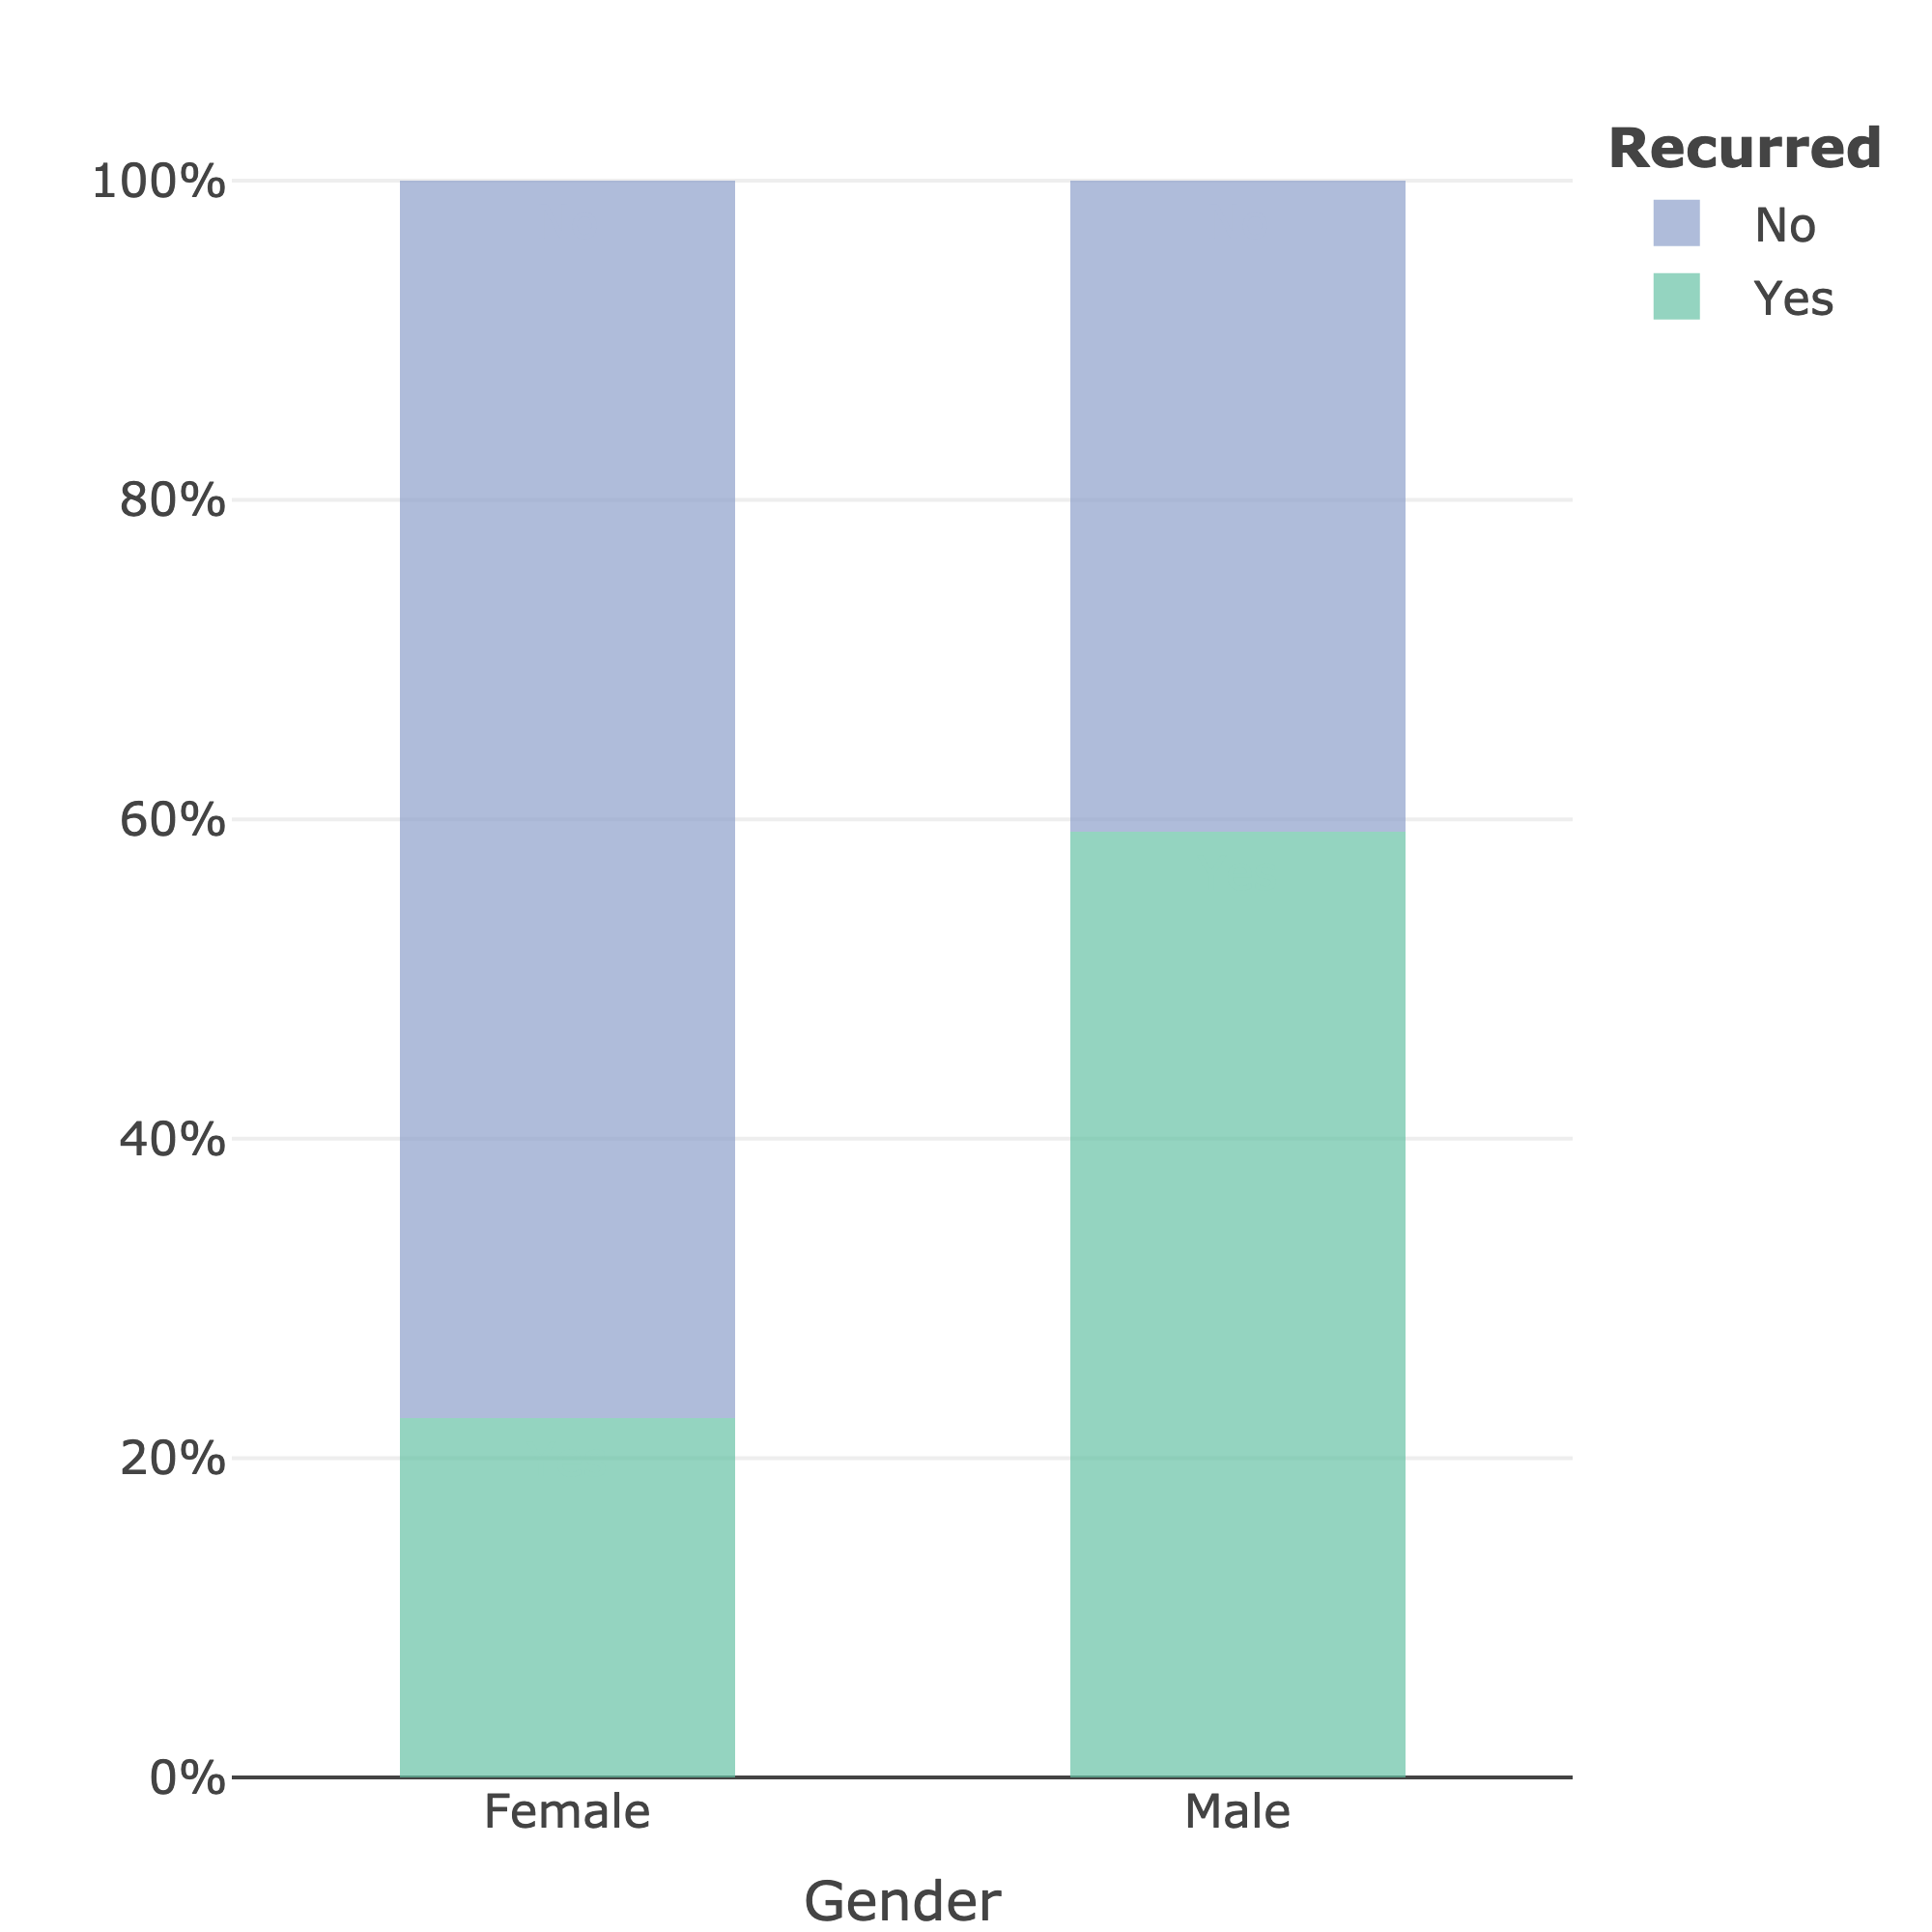
\includegraphics[width=4.375in,height=\textheight]{images/gender_dist_plot.png}

}

\caption{\label{fig-gender-dist}Gender Distribution by Cancer
Recurrence.}

\end{figure}%

The distribution of \texttt{Age} by cancer recurrence is shown in
Figure~\ref{fig-age-dist}. Note that, in general, older patients are
more likely to recur.

\phantomsection\label{cell-fig-age-dist}
\begin{figure}[H]

\centering{

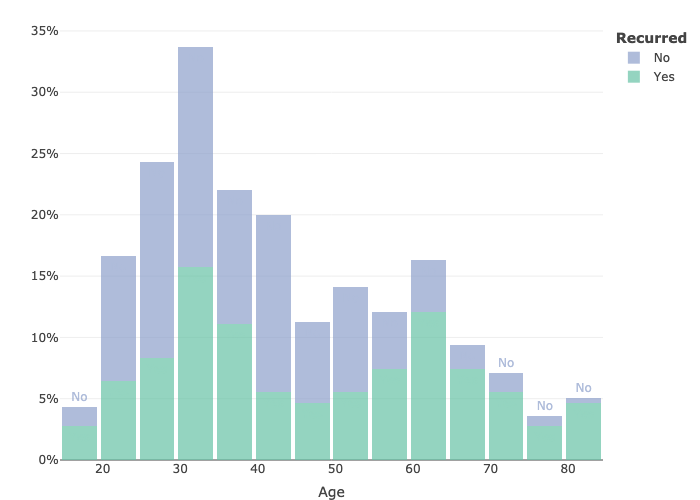
\includegraphics[width=4.375in,height=\textheight]{images/age_dist_plot.png}

}

\caption{\label{fig-age-dist}Age Distribution by Cancer Recurrence}

\end{figure}%

Besides \texttt{Age}, the rest of the features are categorical. One
interesting categorical feature is \texttt{Adenopathy}. It represents
the presence of swollen lymph nodes during physical examination. The
different adenopathy types observed are no adenopathy, anterior right,
anterior left, bilateral (i.e., both sides of the body), posterior, and
extensive (i.e., involves all the locations). Note the high correlation
between swollen lymph nodes and DTC recurrence rate (see
Figure~\ref{fig-aden-dist}).

\phantomsection\label{cell-fig-aden-dist}
\begin{figure}[H]

\centering{

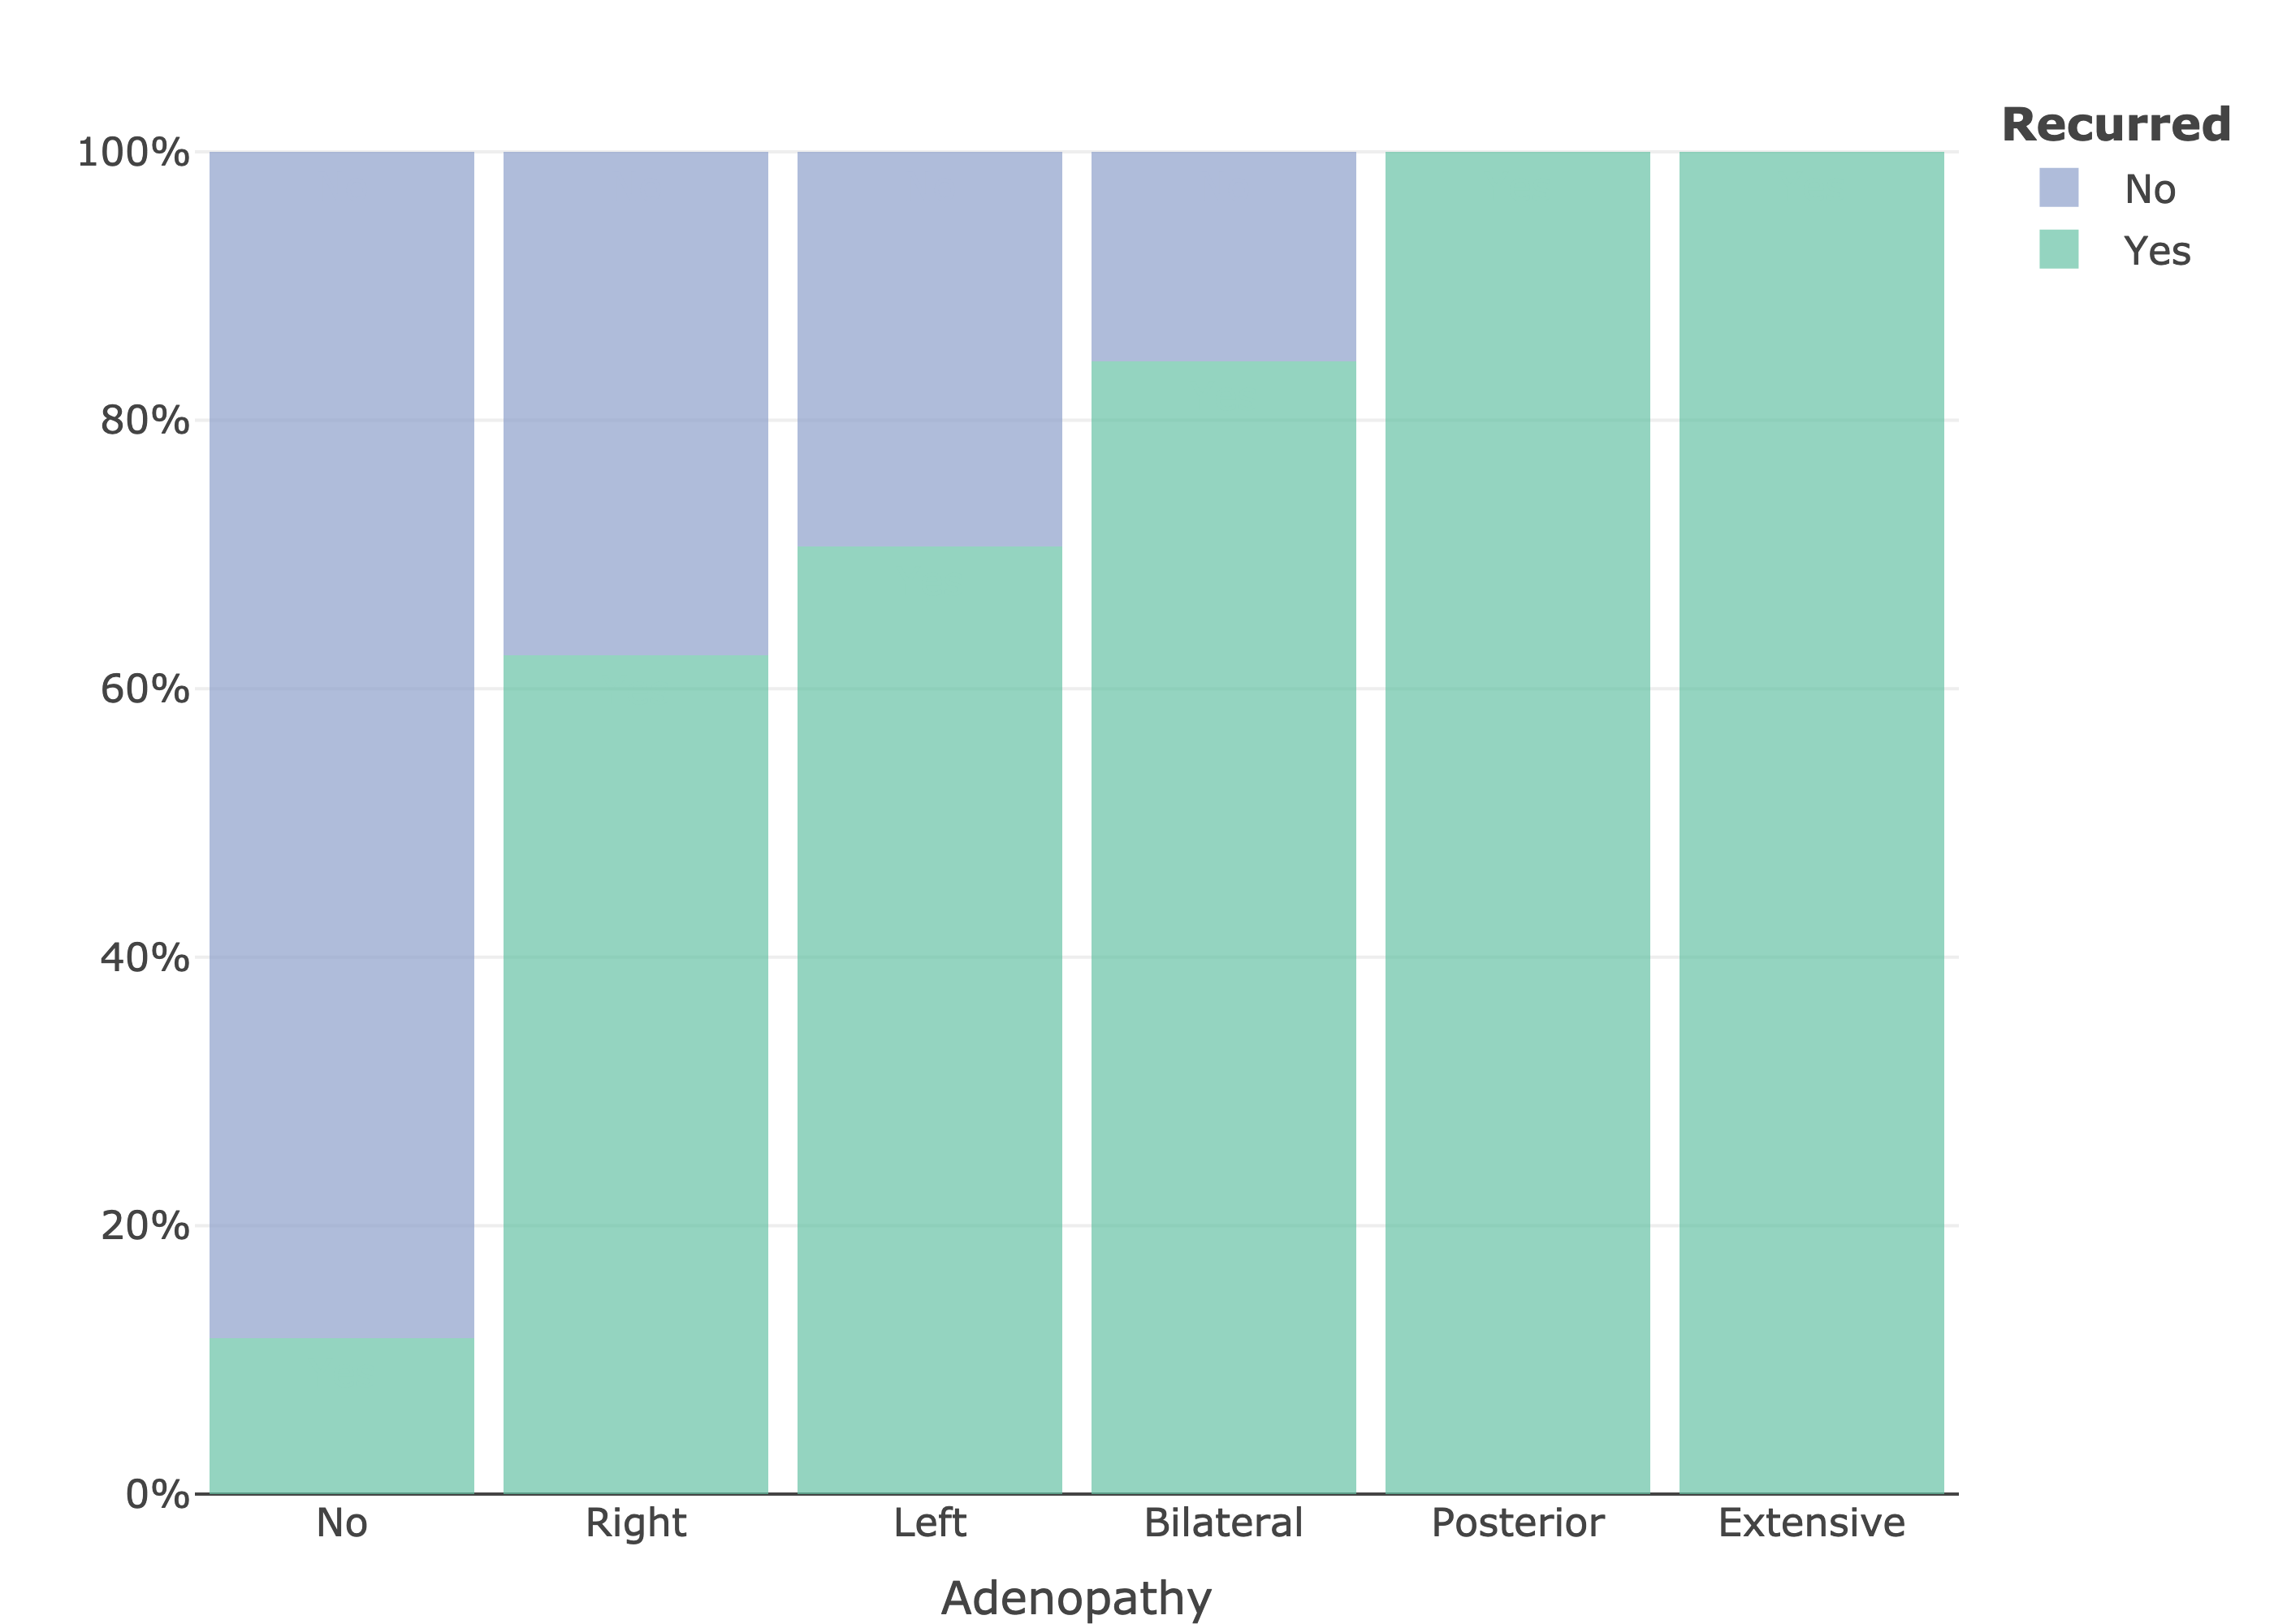
\includegraphics[width=4.375in,height=\textheight]{images/aden_dist_plot.png}

}

\caption{\label{fig-aden-dist}Adenopathy Distribution by cancer
recurrence.}

\end{figure}%

A summary of all the features and their categories are shown in
Table~\ref{tbl-summary}.

\begin{longtable}{>{\raggedright\arraybackslash}p{\dimexpr 0.5\linewidth-2\tabcolsep-1.5\arrayrulewidth}>{\raggedright\arraybackslash}p{\dimexpr 0.5\linewidth-2\tabcolsep-1.5\arrayrulewidth}}

\caption{\label{tbl-summary}Feature Names and their Distinct Values}

\tabularnewline

\toprule
Feature & Values \\ 
\midrule\addlinespace[2.5pt]
\cellcolor[HTML]{FFFFFF}{Gender} & \cellcolor[HTML]{FFFFFF}{Female, Male} \\ 
\cellcolor[HTML]{FFFFFF}{Smoking} & \cellcolor[HTML]{FFFFFF}{Yes, No} \\ 
\cellcolor[HTML]{FFFFFF}{Hx Smoking} & \cellcolor[HTML]{FFFFFF}{Yes, No} \\ 
\cellcolor[HTML]{FFFFFF}{Hx Radiotherapy} & \cellcolor[HTML]{FFFFFF}{Yes, No} \\ 
\cellcolor[HTML]{FFFFFF}{Thyroid Function} & \cellcolor[HTML]{FFFFFF}{Euthyroid, Clinical Hyperthyroidism, Subclinical Hyperthyroidism, Clinical Hypothyroidism, Subclinical Hypothyroidism} \\ 
\cellcolor[HTML]{FFFFFF}{Physical Examination} & \cellcolor[HTML]{FFFFFF}{Normal, Diffuse goiter, Single nodular goiter-right, Single nodular goiter-left, Multinodular goiter} \\ 
\cellcolor[HTML]{FFFFFF}{Adenopathy} & \cellcolor[HTML]{FFFFFF}{No, Right, Left, Bilateral, Posterior, Extensive} \\ 
\cellcolor[HTML]{FFFFFF}{Pathology} & \cellcolor[HTML]{FFFFFF}{Papillary, Micropapillary, Follicular, Hurthel cell} \\ 
\cellcolor[HTML]{FFFFFF}{Focality} & \cellcolor[HTML]{FFFFFF}{Uni-Focal, Multi-Focal} \\ 
\cellcolor[HTML]{FFFFFF}{Risk} & \cellcolor[HTML]{FFFFFF}{Low, Intermediate, High} \\ 
\cellcolor[HTML]{FFFFFF}{T} & \cellcolor[HTML]{FFFFFF}{T1a, T1b, T2, T3a, T3b, T4a, T4b} \\ 
\cellcolor[HTML]{FFFFFF}{N} & \cellcolor[HTML]{FFFFFF}{N0, N1b, N1a} \\ 
\cellcolor[HTML]{FFFFFF}{M} & \cellcolor[HTML]{FFFFFF}{M0, M1} \\ 
\cellcolor[HTML]{FFFFFF}{Stage} & \cellcolor[HTML]{FFFFFF}{I, II, III, IVA, IVB} \\ 
\cellcolor[HTML]{FFFFFF}{Response} & \cellcolor[HTML]{FFFFFF}{Excellent, Biochemical Incomplete, Structural Incomplete, Indeterminate} \\ 
\bottomrule

\end{longtable}

\section{Model Training}\label{model-training}

Let us split the cleaned data set into a training (\(75\%\)) set and a
test (\(25\%\)) set using a random generator. The training data will be
further separated into 10 folds for cross-validation.

\begin{Shaded}
\begin{Highlighting}[]
\CommentTok{\# Split data into training and test sets.}
\FunctionTok{set.seed}\NormalTok{(}\DecValTok{314}\NormalTok{)}
\NormalTok{data\_split }\OtherTok{\textless{}{-}}\NormalTok{ rsample}\SpecialCharTok{::}\FunctionTok{initial\_split}\NormalTok{(cleaned\_data)}
\NormalTok{train\_data }\OtherTok{\textless{}{-}}\NormalTok{ rsample}\SpecialCharTok{::}\FunctionTok{training}\NormalTok{(data\_split)}
\NormalTok{test\_data }\OtherTok{\textless{}{-}}\NormalTok{ rsample}\SpecialCharTok{::}\FunctionTok{testing}\NormalTok{(data\_split)}

\CommentTok{\# Split the training data into 10{-}folds for cross{-}validation.}
\FunctionTok{set.seed}\NormalTok{(}\DecValTok{3145}\NormalTok{)}
\NormalTok{data\_cross\_val }\OtherTok{\textless{}{-}}\NormalTok{ rsample}\SpecialCharTok{::}\FunctionTok{vfold\_cv}\NormalTok{(train\_data)}

\CommentTok{\# Set aside the outcome column of the sample test data.}
\NormalTok{test\_outcome }\OtherTok{\textless{}{-}} \FunctionTok{factor}\NormalTok{(test\_data}\SpecialCharTok{$}\NormalTok{Recurred)}
\end{Highlighting}
\end{Shaded}

The \texttt{recipes} package is useful to create a blueprint of the
pre-processing steps that will be applied to our data during model
training. We use this package to specify that

\begin{itemize}
\tightlist
\item
  the minimum number of features with absolute correlations less that
  \(0.6\) should be removed,
\item
  the numeric features should be normalized, and
\item
  the categorical variables should be transformed into numerical
  variables.
\end{itemize}

\begin{Shaded}
\begin{Highlighting}[]
\CommentTok{\# Create recipe for the data prep.}
\NormalTok{data\_rec }\OtherTok{\textless{}{-}}\NormalTok{ recipes}\SpecialCharTok{::}\FunctionTok{recipe}\NormalTok{(Recurred }\SpecialCharTok{\textasciitilde{}}\NormalTok{ ., }\AttributeTok{data =}\NormalTok{ train\_data) }\SpecialCharTok{|\textgreater{}}
\NormalTok{  recipes}\SpecialCharTok{::}\FunctionTok{step\_corr}\NormalTok{(}\AttributeTok{threshold =} \FloatTok{0.6}\NormalTok{) }\SpecialCharTok{|\textgreater{}}
\NormalTok{  recipes}\SpecialCharTok{::}\FunctionTok{step\_normalize}\NormalTok{(recipes}\SpecialCharTok{::}\FunctionTok{all\_numeric}\NormalTok{()) }\SpecialCharTok{|\textgreater{}}
\NormalTok{  recipes}\SpecialCharTok{::}\FunctionTok{step\_dummy}\NormalTok{(recipes}\SpecialCharTok{::}\FunctionTok{all\_nominal\_predictors}\NormalTok{())}
\end{Highlighting}
\end{Shaded}

\subsection{K-Nearest Neighbors}\label{k-nearest-neighbors}

\subsubsection{Model Description}\label{model-description}

The K-Nearest Neighbors (KNN) algorithm is a nonparametric method used
for classification. It classifies a given sample based on the proximity
to the training data. The algorithm determines the class of a point
\(X\) by identifying the most common class label among its \(k\) nearest
neighbors, where \(k\) is a predetermined hyperparameter. Unlike other
algorithms, the KNN classifier does not involve training a model;
instead, it memorizes the training data, making it a ``lazy'' algorithm.

The primary hyperparameters of the KNN algorithm are \(k\), the distance
measure, and the weight function. Common distance measures include
Euclidean distance, Manhattan distance, and Minkowski distance.

Choosing the optimal value for \(k\) is crucial and involves balancing
the bias-variance tradeoff. A small \(k\) results in low bias and high
variance. Low bias means the model captures the complexity of the
training data very well, but high variance means the model is highly
sensitive to the specifics of the training data, often leading to
overfitting and higher test errors. As \(k\) increases, the model
averages over more neighbors, which smooths out the predictions and
reduces the model's sensitivity to individual data points, thus reducing
variance. Therefore, a large \(k\) results in high bias and low
variance. The model may become too simplistic, leading to higher bias,
but it becomes less sensitive to the training data, making it more
robust to noise and better at generalizing to new data.

To avoid classification ties, it is advisable to select \(k\)
appropriately. For binary classification, this typically means choosing
an odd \(k\). Additionally, to enhance model flexibility, a weighted
version of KNN can be employed, where the influence of each of the \(k\)
nearest neighbors is weighted inversely by their distance to the test
point. We will tune these three parameters below.

\subsubsection{Model Workflow}\label{model-workflow}

Below we create a KNN model specification and workflow indicating the
model hyperparameters: a number of neighbors (i.e., \(k\)), a weight
function, and a distance function. To optimize our model, we will use
the \texttt{tune::tune()} function to find optimal values of these
parameters based on model accuracy.

\begin{Shaded}
\begin{Highlighting}[]
\CommentTok{\# Create model specification.}
\NormalTok{knn\_model\_spec }\OtherTok{\textless{}{-}}
\NormalTok{  parsnip}\SpecialCharTok{::}\FunctionTok{nearest\_neighbor}\NormalTok{(}
    \AttributeTok{neighbors =}\NormalTok{ tune}\SpecialCharTok{::}\FunctionTok{tune}\NormalTok{(),}
    \AttributeTok{dist\_power =}\NormalTok{ tune}\SpecialCharTok{::}\FunctionTok{tune}\NormalTok{(),}
    \AttributeTok{weight\_func =}\NormalTok{ tune}\SpecialCharTok{::}\FunctionTok{tune}\NormalTok{()}
\NormalTok{  ) }\SpecialCharTok{|\textgreater{}}
\NormalTok{  parsnip}\SpecialCharTok{::}\FunctionTok{set\_mode}\NormalTok{(}\StringTok{\textquotesingle{}classification\textquotesingle{}}\NormalTok{) }\SpecialCharTok{|\textgreater{}}
\NormalTok{  parsnip}\SpecialCharTok{::}\FunctionTok{set\_engine}\NormalTok{(}\StringTok{\textquotesingle{}kknn\textquotesingle{}}\NormalTok{)}

\CommentTok{\# Create model workflow.}
\NormalTok{knn\_workflow }\OtherTok{\textless{}{-}}\NormalTok{ workflows}\SpecialCharTok{::}\FunctionTok{workflow}\NormalTok{() }\SpecialCharTok{|\textgreater{}}
\NormalTok{  workflows}\SpecialCharTok{::}\FunctionTok{add\_model}\NormalTok{(knn\_model\_spec) }\SpecialCharTok{|\textgreater{}}
\NormalTok{  workflows}\SpecialCharTok{::}\FunctionTok{add\_recipe}\NormalTok{(data\_rec)}
\end{Highlighting}
\end{Shaded}

\subsubsection{Model Tuning and Fitting}\label{model-tuning-and-fitting}

Next, we run our prepared workflow. To speed up the computation, we
utilize parallel computing, distributing the tasks across multiple
cores.

We fine-tune the model hyperparameters (namely \(k\), the distance
function, and the weight function) using the \(10\)-fold
cross-validation setup. We then select the best model based on accuracy.

\begin{Shaded}
\begin{Highlighting}[]
\CommentTok{\#\textquotesingle{} Check number of available cores.}
\NormalTok{cores\_no }\OtherTok{\textless{}{-}}\NormalTok{ parallel}\SpecialCharTok{::}\FunctionTok{detectCores}\NormalTok{() }\SpecialCharTok{{-}} \DecValTok{1}

\CommentTok{\#\textquotesingle{} Start timer.}
\NormalTok{tictoc}\SpecialCharTok{::}\FunctionTok{tic}\NormalTok{()}

\CommentTok{\# Create and register clusters.}
\NormalTok{clusters }\OtherTok{\textless{}{-}}\NormalTok{ parallel}\SpecialCharTok{::}\FunctionTok{makeCluster}\NormalTok{(cores\_no)}
\NormalTok{doParallel}\SpecialCharTok{::}\FunctionTok{registerDoParallel}\NormalTok{(clusters)}

\CommentTok{\# Fine{-}tune the model params.}
\NormalTok{knn\_res }\OtherTok{\textless{}{-}}\NormalTok{ tune}\SpecialCharTok{::}\FunctionTok{tune\_grid}\NormalTok{(}
  \AttributeTok{object =}\NormalTok{ knn\_workflow,}
  \AttributeTok{resamples =}\NormalTok{ data\_cross\_val,}
  \AttributeTok{control =}\NormalTok{ tune}\SpecialCharTok{::}\FunctionTok{control\_resamples}\NormalTok{(}\AttributeTok{save\_pred =} \ConstantTok{TRUE}\NormalTok{)}
\NormalTok{)}

\CommentTok{\# Select the best fit based on accuracy.}
\NormalTok{knn\_best\_fit }\OtherTok{\textless{}{-}} 
\NormalTok{  knn\_res }\SpecialCharTok{|\textgreater{}} 
\NormalTok{  tune}\SpecialCharTok{::}\FunctionTok{select\_best}\NormalTok{(}\AttributeTok{metric =} \StringTok{\textquotesingle{}accuracy\textquotesingle{}}\NormalTok{)}

\CommentTok{\# Finalize the workflow with the best parameters.}
\NormalTok{knn\_final\_workflow }\OtherTok{\textless{}{-}} 
\NormalTok{  knn\_workflow }\SpecialCharTok{|\textgreater{}}
\NormalTok{  tune}\SpecialCharTok{::}\FunctionTok{finalize\_workflow}\NormalTok{(knn\_best\_fit)}

\CommentTok{\# Fit the final model using the best parameters.}
\NormalTok{knn\_final\_fit }\OtherTok{\textless{}{-}} 
\NormalTok{  knn\_final\_workflow }\SpecialCharTok{|\textgreater{}} 
\NormalTok{  tune}\SpecialCharTok{::}\FunctionTok{last\_fit}\NormalTok{(data\_split)}

\CommentTok{\# Stop clusters.}
\NormalTok{parallel}\SpecialCharTok{::}\FunctionTok{stopCluster}\NormalTok{(clusters)}

\CommentTok{\# Stop timer.}
\NormalTok{tictoc}\SpecialCharTok{::}\FunctionTok{toc}\NormalTok{()}
\end{Highlighting}
\end{Shaded}

\begin{verbatim}
13.605 sec elapsed
\end{verbatim}

\subsubsection{Model Performance}\label{model-performance}

We then apply our selected model to the test set. The final metrics are
given in Table~\ref{tbl-knn-performance}.

\begin{Shaded}
\begin{Highlighting}[]
\CommentTok{\# Use the best fit to make predictions on the test data.}
\NormalTok{knn\_pred }\OtherTok{\textless{}{-}} 
\NormalTok{  knn\_final\_fit }\SpecialCharTok{|\textgreater{}} 
\NormalTok{  tune}\SpecialCharTok{::}\FunctionTok{collect\_predictions}\NormalTok{() }\SpecialCharTok{|\textgreater{}}
\NormalTok{  dplyr}\SpecialCharTok{::}\FunctionTok{mutate}\NormalTok{(}\AttributeTok{truth =} \FunctionTok{factor}\NormalTok{(.pred\_class))}
\end{Highlighting}
\end{Shaded}

\begin{longtable}{>{\raggedright\arraybackslash}p{\dimexpr 0.5\linewidth-2\tabcolsep-1.5\arrayrulewidth}>{\raggedleft\arraybackslash}p{\dimexpr 0.5\linewidth-2\tabcolsep-1.5\arrayrulewidth}}

\caption{\label{tbl-knn-performance}KNN Performance Metrics: Accuracy,
Precision, Recall, and Specificity.}

\tabularnewline

\toprule
Metric & Value \\ 
\midrule\addlinespace[2.5pt]
\cellcolor[HTML]{FFFFFF}{Accuracy} & \cellcolor[HTML]{FFFFFF}{90.1} \\ 
\cellcolor[HTML]{FFFFFF}{Precision} & \cellcolor[HTML]{FFFFFF}{76.9} \\ 
\cellcolor[HTML]{FFFFFF}{Recall} & \cellcolor[HTML]{FFFFFF}{87.0} \\ 
\cellcolor[HTML]{FFFFFF}{Specificity} & \cellcolor[HTML]{FFFFFF}{91.2} \\ 
\bottomrule

\end{longtable}

\subsection{Support Vector Machine}\label{support-vector-machine}

\subsubsection{Model Description}\label{model-description-1}

Support Vector Machines (SVM) are powerful supervised learning
algorithms used for both classification and regression tasks. For
classification, SVM works by finding the hyperplane that best separates
data points of different classes in a high-dimensional space. The
optimal hyperplane is determined by maximizing the margin between the
closest points of the classes, known as support vectors.

SVM is particularly effective in high-dimensional spaces and is useful
when the number of dimensions exceeds the number of samples. It can
employ various kernel functions---such as linear, polynomial, and radial
basis function (RBF)---to handle non-linear classification by mapping
input features into higher-dimensional spaces.

The most commonly used kernel in SVM is the Radial Basis Function (RBF)
kernel, also known as the Gaussian kernel. The RBF kernel maps input
features into an infinite-dimensional space, allowing SVM to create
complex decision boundaries. The RBF kernel function is defined as:

\[K(X_i, X_j) = e^{- \frac{|| X_i - X_j ||^2}{2 \sigma^2}}\] where
\(X_i\) and \(X_j\) are the input feature vectors, and \(\sigma\) is a
parameter that determines the spread of the kernel and controls the
influence of individual training samples.

\subsubsection{Model Workflow}\label{model-workflow-1}

We will create an SVM model specification and workflow, indicating the
model hyperparameters \(\sigma\) (or \texttt{rbf\_sigma}) and
\texttt{cost}. The \texttt{rbf\_sigma} parameter controls the influence
of individual training examples, while the \texttt{cost} parameter
controls the trade-off between achieving a low training error and a low
testing error, which affects the model's ability to generalize. To
optimize our model, we will use the \texttt{tune::tune()} function to
find the optimal values of these parameters in terms of model accuracy.

\begin{Shaded}
\begin{Highlighting}[]
\CommentTok{\# Create model specification.}
\NormalTok{svm\_model\_spec }\OtherTok{\textless{}{-}}
\NormalTok{  parsnip}\SpecialCharTok{::}\FunctionTok{svm\_rbf}\NormalTok{(}
    \AttributeTok{cost =}\NormalTok{ tune}\SpecialCharTok{::}\FunctionTok{tune}\NormalTok{(),}
    \AttributeTok{rbf\_sigma =}\NormalTok{ tune}\SpecialCharTok{::}\FunctionTok{tune}\NormalTok{()}
\NormalTok{  ) }\SpecialCharTok{|\textgreater{}}
\NormalTok{  parsnip}\SpecialCharTok{::}\FunctionTok{set\_engine}\NormalTok{(}\StringTok{\textquotesingle{}kernlab\textquotesingle{}}\NormalTok{) }\SpecialCharTok{|\textgreater{}}
\NormalTok{  parsnip}\SpecialCharTok{::}\FunctionTok{set\_mode}\NormalTok{(}\StringTok{\textquotesingle{}classification\textquotesingle{}}\NormalTok{)}

\CommentTok{\# Create model workflow.}
\NormalTok{svm\_workflow }\OtherTok{\textless{}{-}}\NormalTok{ workflows}\SpecialCharTok{::}\FunctionTok{workflow}\NormalTok{() }\SpecialCharTok{|\textgreater{}}
\NormalTok{  workflows}\SpecialCharTok{::}\FunctionTok{add\_model}\NormalTok{(svm\_model\_spec) }\SpecialCharTok{|\textgreater{}}
\NormalTok{  workflows}\SpecialCharTok{::}\FunctionTok{add\_recipe}\NormalTok{(data\_rec)}
\end{Highlighting}
\end{Shaded}

\subsubsection{Model Tuning and
Fitting}\label{model-tuning-and-fitting-1}

As we did for KNN, we use parallel computing to fine-tuning our model
using the \(10\)-fold cross-validation we set up earlier. We end this
section by selecting the best model based on accuracy.

\begin{Shaded}
\begin{Highlighting}[]
\CommentTok{\#\textquotesingle{} Check number of available cores.}
\NormalTok{cores\_no }\OtherTok{\textless{}{-}}\NormalTok{ parallel}\SpecialCharTok{::}\FunctionTok{detectCores}\NormalTok{() }\SpecialCharTok{{-}} \DecValTok{1}

\CommentTok{\#\textquotesingle{} Start timer.}
\NormalTok{tictoc}\SpecialCharTok{::}\FunctionTok{tic}\NormalTok{()}

\CommentTok{\# Create and register clusters.}
\NormalTok{clusters }\OtherTok{\textless{}{-}}\NormalTok{ parallel}\SpecialCharTok{::}\FunctionTok{makeCluster}\NormalTok{(cores\_no)}
\NormalTok{doParallel}\SpecialCharTok{::}\FunctionTok{registerDoParallel}\NormalTok{(clusters)}

\CommentTok{\# Fine{-}tune the model params.}
\NormalTok{svm\_res }\OtherTok{\textless{}{-}}\NormalTok{ tune}\SpecialCharTok{::}\FunctionTok{tune\_grid}\NormalTok{(}
  \AttributeTok{object =}\NormalTok{ svm\_workflow,}
  \AttributeTok{resamples =}\NormalTok{ data\_cross\_val,}
  \AttributeTok{control =}\NormalTok{ tune}\SpecialCharTok{::}\FunctionTok{control\_resamples}\NormalTok{(}\AttributeTok{save\_pred =} \ConstantTok{TRUE}\NormalTok{)}
\NormalTok{)}

\CommentTok{\# Select the best fit based on accuracy.}
\NormalTok{svm\_best\_fit }\OtherTok{\textless{}{-}} 
\NormalTok{  svm\_res }\SpecialCharTok{|\textgreater{}} 
\NormalTok{  tune}\SpecialCharTok{::}\FunctionTok{select\_best}\NormalTok{(}\AttributeTok{metric =} \StringTok{\textquotesingle{}accuracy\textquotesingle{}}\NormalTok{)}

\CommentTok{\# Finalize the workflow with the best parameters.}
\NormalTok{svm\_final\_workflow }\OtherTok{\textless{}{-}} 
\NormalTok{  svm\_workflow }\SpecialCharTok{|\textgreater{}}
\NormalTok{  tune}\SpecialCharTok{::}\FunctionTok{finalize\_workflow}\NormalTok{(svm\_best\_fit)}

\CommentTok{\# Fit the final model using the best parameters.}
\NormalTok{svm\_final\_fit }\OtherTok{\textless{}{-}} 
\NormalTok{  svm\_final\_workflow }\SpecialCharTok{|\textgreater{}} 
\NormalTok{  tune}\SpecialCharTok{::}\FunctionTok{last\_fit}\NormalTok{(data\_split)}

\CommentTok{\# Stop clusters.}
\NormalTok{parallel}\SpecialCharTok{::}\FunctionTok{stopCluster}\NormalTok{(clusters)}

\CommentTok{\# Stop timer.}
\NormalTok{tictoc}\SpecialCharTok{::}\FunctionTok{toc}\NormalTok{()}
\end{Highlighting}
\end{Shaded}

\begin{verbatim}
18.265 sec elapsed
\end{verbatim}

\subsubsection{Model Performance}\label{model-performance-1}

We then apply our selected model to the test set. The final metrics are
given in Table~\ref{tbl-svm-performance}.

\begin{Shaded}
\begin{Highlighting}[]
\CommentTok{\# Use the best fit to make predictions on the test data.}
\NormalTok{svm\_pred }\OtherTok{\textless{}{-}} 
\NormalTok{  svm\_final\_fit }\SpecialCharTok{|\textgreater{}} 
\NormalTok{  tune}\SpecialCharTok{::}\FunctionTok{collect\_predictions}\NormalTok{() }\SpecialCharTok{|\textgreater{}}
\NormalTok{  dplyr}\SpecialCharTok{::}\FunctionTok{mutate}\NormalTok{(}\AttributeTok{truth =} \FunctionTok{factor}\NormalTok{(.pred\_class))}
\end{Highlighting}
\end{Shaded}

\begin{longtable}{>{\raggedright\arraybackslash}p{\dimexpr 0.5\linewidth-2\tabcolsep-1.5\arrayrulewidth}>{\raggedleft\arraybackslash}p{\dimexpr 0.5\linewidth-2\tabcolsep-1.5\arrayrulewidth}}

\caption{\label{tbl-svm-performance}SVM Performance Metrics: Accuracy,
Precision, Recall, and Specificity.}

\tabularnewline

\toprule
Metric & Value \\ 
\midrule\addlinespace[2.5pt]
\cellcolor[HTML]{FFFFFF}{Accuracy} & \cellcolor[HTML]{FFFFFF}{78.0} \\ 
\cellcolor[HTML]{FFFFFF}{Precision} & \cellcolor[HTML]{FFFFFF}{23.1} \\ 
\cellcolor[HTML]{FFFFFF}{Recall} & \cellcolor[HTML]{FFFFFF}{100.0} \\ 
\cellcolor[HTML]{FFFFFF}{Specificity} & \cellcolor[HTML]{FFFFFF}{76.5} \\ 
\bottomrule

\end{longtable}

\subsection{Artificial Neural Network}\label{artificial-neural-network}

\subsubsection{Model Description}\label{model-description-2}

Artificial Neural Networks (ANNs) are a class of machine learning
algorithms inspired by the structure and function of the human brain.
They consist of interconnected layers of nodes, or neurons, which
process input data to perform tasks such as classification, regression,
and pattern recognition. ANNs are particularly effective for complex
tasks like image and speech recognition, natural language processing,
financial forecasting, and medical diagnosis.

An ANN is composed of multiple layers, including an input layer, one or
more hidden layers, and an output layer. The input layer receives the
raw data, the hidden layers process the data through various
transformations, and the output layer produces the final prediction or
classification. Each connection between neurons has an associated
weight, and each neuron has a bias term. These parameters are adjusted
during the training process to minimize the error in predictions.

The training process of an ANN involves forward propagation, where input
data is passed through the network layer by layer. Each neuron applies
an activation function to compute its output, introducing non-linearity
to help the network learn complex patterns. The loss, or error, between
the network's output and the true target values is calculated using a
loss function. Through backpropagation, the loss is propagated backward
through the network, and the weights and biases are adjusted using an
optimization algorithm like gradient descent.

ANNs offer significant advantages, including flexibility in modeling
complex relationships and scalability to handle large datasets and
intricate tasks. Their ability to learn and generalize from data makes
them powerful tools in various applications, driving advancements in
fields ranging from technology and finance to healthcare and beyond.

\subsubsection{Model Workflow}\label{model-workflow-2}

Let us start by specifying the ANN model and creating the model
workflow. Specifically, we will define a multilayer perceptron model
(i.e., a single-layer, feed-forward neural network). The key parameters
we will set include the number of epochs (or training iterations), the
number of hidden units, the penalty (or weight decay), and the learning
rate.

\begin{Shaded}
\begin{Highlighting}[]
\CommentTok{\# Create model specification.}
\NormalTok{ann\_model\_spec }\OtherTok{\textless{}{-}}
\NormalTok{  parsnip}\SpecialCharTok{::}\FunctionTok{mlp}\NormalTok{(}
    \AttributeTok{epochs =}\NormalTok{ tune}\SpecialCharTok{::}\FunctionTok{tune}\NormalTok{(),}
    \AttributeTok{hidden\_units =}\NormalTok{ tune}\SpecialCharTok{::}\FunctionTok{tune}\NormalTok{(),}
    \AttributeTok{penalty =}\NormalTok{ tune}\SpecialCharTok{::}\FunctionTok{tune}\NormalTok{(),}
    \AttributeTok{learn\_rate =} \FloatTok{0.1}
\NormalTok{  ) }\SpecialCharTok{|\textgreater{}}
\NormalTok{  parsnip}\SpecialCharTok{::}\FunctionTok{set\_engine}\NormalTok{(}\StringTok{\textquotesingle{}nnet\textquotesingle{}}\NormalTok{) }\SpecialCharTok{|\textgreater{}}
\NormalTok{  parsnip}\SpecialCharTok{::}\FunctionTok{set\_mode}\NormalTok{(}\StringTok{\textquotesingle{}classification\textquotesingle{}}\NormalTok{)}

\CommentTok{\# Create model workflow.}
\NormalTok{ann\_workflow }\OtherTok{\textless{}{-}}\NormalTok{ workflows}\SpecialCharTok{::}\FunctionTok{workflow}\NormalTok{() }\SpecialCharTok{|\textgreater{}}
\NormalTok{  workflows}\SpecialCharTok{::}\FunctionTok{add\_model}\NormalTok{(ann\_model\_spec) }\SpecialCharTok{|\textgreater{}}
\NormalTok{  workflows}\SpecialCharTok{::}\FunctionTok{add\_recipe}\NormalTok{(data\_rec)}
\end{Highlighting}
\end{Shaded}

\subsubsection{Model Tuning and
Fitting}\label{model-tuning-and-fitting-2}

We will proceed to tune all the parameters except for the learning rate.
This is because the \texttt{nnet} package does not support tuning the
learning rate.

\begin{Shaded}
\begin{Highlighting}[]
\CommentTok{\#\textquotesingle{} Check number of available cores.}
\NormalTok{cores\_no }\OtherTok{\textless{}{-}}\NormalTok{ parallel}\SpecialCharTok{::}\FunctionTok{detectCores}\NormalTok{() }\SpecialCharTok{{-}} \DecValTok{1}

\CommentTok{\#\textquotesingle{} Start timer.}
\NormalTok{tictoc}\SpecialCharTok{::}\FunctionTok{tic}\NormalTok{()}

\CommentTok{\# Create and register clusters.}
\NormalTok{clusters }\OtherTok{\textless{}{-}}\NormalTok{ parallel}\SpecialCharTok{::}\FunctionTok{makeCluster}\NormalTok{(cores\_no)}
\NormalTok{doParallel}\SpecialCharTok{::}\FunctionTok{registerDoParallel}\NormalTok{(clusters)}

\CommentTok{\# Fine{-}tune the model params.}
\NormalTok{ann\_res }\OtherTok{\textless{}{-}}\NormalTok{ tune}\SpecialCharTok{::}\FunctionTok{tune\_grid}\NormalTok{(}
  \AttributeTok{object =}\NormalTok{ ann\_workflow,}
  \AttributeTok{resamples =}\NormalTok{ data\_cross\_val,}
  \AttributeTok{control =}\NormalTok{ tune}\SpecialCharTok{::}\FunctionTok{control\_resamples}\NormalTok{(}\AttributeTok{save\_pred =} \ConstantTok{TRUE}\NormalTok{)}
\NormalTok{)}

\CommentTok{\# Select the best fit based on accuracy.}
\NormalTok{ann\_best\_fit }\OtherTok{\textless{}{-}} 
\NormalTok{  ann\_res }\SpecialCharTok{|\textgreater{}} 
\NormalTok{  tune}\SpecialCharTok{::}\FunctionTok{select\_best}\NormalTok{(}\AttributeTok{metric =} \StringTok{\textquotesingle{}accuracy\textquotesingle{}}\NormalTok{)}

\CommentTok{\# Finalize the workflow with the best parameters.}
\NormalTok{ann\_final\_workflow }\OtherTok{\textless{}{-}} 
\NormalTok{  ann\_workflow }\SpecialCharTok{|\textgreater{}}
\NormalTok{  tune}\SpecialCharTok{::}\FunctionTok{finalize\_workflow}\NormalTok{(ann\_best\_fit)}

\CommentTok{\# Fit the final model using the best parameters.}
\NormalTok{ann\_final\_fit }\OtherTok{\textless{}{-}} 
\NormalTok{  ann\_final\_workflow }\SpecialCharTok{|\textgreater{}} 
\NormalTok{  tune}\SpecialCharTok{::}\FunctionTok{last\_fit}\NormalTok{(data\_split)}

\CommentTok{\# Stop clusters.}
\NormalTok{parallel}\SpecialCharTok{::}\FunctionTok{stopCluster}\NormalTok{(clusters)}

\CommentTok{\# Stop timer.}
\NormalTok{tictoc}\SpecialCharTok{::}\FunctionTok{toc}\NormalTok{()}
\end{Highlighting}
\end{Shaded}

\begin{verbatim}
13.78 sec elapsed
\end{verbatim}

\subsubsection{Model Performance}\label{model-performance-2}

We then apply our selected model to the test set. The final metrics are
given in Table~\ref{tbl-ann-performance}.

\begin{Shaded}
\begin{Highlighting}[]
\CommentTok{\# Use the best fit to make predictions on the test data.}
\NormalTok{ann\_pred }\OtherTok{\textless{}{-}} 
\NormalTok{  ann\_final\_fit }\SpecialCharTok{|\textgreater{}} 
\NormalTok{  tune}\SpecialCharTok{::}\FunctionTok{collect\_predictions}\NormalTok{() }\SpecialCharTok{|\textgreater{}}
\NormalTok{  dplyr}\SpecialCharTok{::}\FunctionTok{mutate}\NormalTok{(}\AttributeTok{truth =} \FunctionTok{factor}\NormalTok{(.pred\_class))}
\end{Highlighting}
\end{Shaded}

\begin{longtable}{>{\raggedright\arraybackslash}p{\dimexpr 0.5\linewidth-2\tabcolsep-1.5\arrayrulewidth}>{\raggedleft\arraybackslash}p{\dimexpr 0.5\linewidth-2\tabcolsep-1.5\arrayrulewidth}}

\caption{\label{tbl-ann-performance}ANN Performance Metrics: Accuracy,
Precision, Recall, and Specificity.}

\tabularnewline

\toprule
Metric & Value \\ 
\midrule\addlinespace[2.5pt]
\cellcolor[HTML]{FFFFFF}{Accuracy} & \cellcolor[HTML]{FFFFFF}{92.3} \\ 
\cellcolor[HTML]{FFFFFF}{Precision} & \cellcolor[HTML]{FFFFFF}{84.6} \\ 
\cellcolor[HTML]{FFFFFF}{Recall} & \cellcolor[HTML]{FFFFFF}{88.0} \\ 
\cellcolor[HTML]{FFFFFF}{Specificity} & \cellcolor[HTML]{FFFFFF}{93.9} \\ 
\bottomrule

\end{longtable}

\subsection{Logistic Regression}\label{logistic-regression}

\subsubsection{Model Description}\label{model-description-3}

Logistic Regression (LR) is a supervised learning algorithm widely used
for classification problems. It is particularly effective for binary
classification tasks, where the outcome variable can take one of two
possible values. The model predicts the probability that a given input
belongs to a specific class by applying the logistic (sigmoid) function,
which transforms a linear combination of input features into a
probability value between \(0\) and \(1\).

For binary classification, the logistic function is defined as
\(\sigma(\hat{Y}_i) = 1/(1 + e^{-\hat{Y}_i})\) where \(\hat{Y}\) is a
linear combination of the input features. The probability of the outcome
\(i\) being the positive class (represented as 1) is given by:

\[\sigma(\hat{Y}_i) = \sigma(\beta_0 + \beta_1 X_{1, i} + \beta_2 X_{2, i} + \ldots + \beta_p X_{p, i}),\]

where \(\beta_0\) is the intercept, and
\(\beta_1, \beta_2, \ldots, \beta_p\) are the coefficients corresponding
to the input features \(X_1, X_2, \ldots, X_p\). These coefficients are
estimated using the method of maximum likelihood estimation (MLE), which
maximizes the likelihood of the observed data.

LR can also be extended to handle multi-class classification problems
through multinomial logistic regression. In this case, the model uses
the softmax function to generalize to multiple classes. The softmax
function is an extension of the logistic function for multiple classes
and is defined as:

\[Pr(Y = j | X = x_0) = \frac{e^{\mathbf{\beta}_j x_0}}{\sum_{i=1}^{n} e^{\mathbf{\beta}_i \cdot x_0}}\]

where \(x_0\) is an observation, \(n\) is the number of classes, and
\(\mathbf{\beta}_j\) is the coefficient vector for class \(j\).

The primary advantage of LR is its interpretability. Each coefficient
indicates the change in the log-odds of the outcome for a one-unit
change in the corresponding predictor variable. This provides clear
insights into the influence of each predictor on the probability of the
outcome. Despite its simplicity, LR is a powerful tool for both binary
and multi-class classification, making it suitable for a wide range of
applications where the relationship between the predictors and the
log-odds is approximately linear.

\subsubsection{Model Workflow}\label{model-workflow-3}

In this section, we will train our LR model and find the optimal values
for the model parameters. The key parameter we will optimize is the
penalty parameter, which refers to the regularization term added to the
loss function to prevent overfitting. We will find the optimal penalty
value to improve model performance. Additionally, we will set mixture =
1 to apply Lasso regularization, which helps in potentially removing
irrelevant predictors and choosing a simpler model.

\begin{Shaded}
\begin{Highlighting}[]
\CommentTok{\# Create model specification.}
\NormalTok{lr\_model\_spec }\OtherTok{\textless{}{-}}
\NormalTok{  parsnip}\SpecialCharTok{::}\FunctionTok{logistic\_reg}\NormalTok{(}
    \AttributeTok{penalty =} \FunctionTok{tune}\NormalTok{(),}
    \AttributeTok{mixture =} \DecValTok{1}\NormalTok{) }\SpecialCharTok{|\textgreater{}}
\NormalTok{  parsnip}\SpecialCharTok{::}\FunctionTok{set\_mode}\NormalTok{(}\StringTok{\textquotesingle{}classification\textquotesingle{}}\NormalTok{) }\SpecialCharTok{|\textgreater{}}
\NormalTok{  parsnip}\SpecialCharTok{::}\FunctionTok{set\_engine}\NormalTok{(}\StringTok{\textquotesingle{}glmnet\textquotesingle{}}\NormalTok{)}

\CommentTok{\# Create model workflow.}
\NormalTok{lr\_workflow }\OtherTok{\textless{}{-}}\NormalTok{ workflows}\SpecialCharTok{::}\FunctionTok{workflow}\NormalTok{() }\SpecialCharTok{|\textgreater{}}
\NormalTok{  workflows}\SpecialCharTok{::}\FunctionTok{add\_model}\NormalTok{(lr\_model\_spec) }\SpecialCharTok{|\textgreater{}}
\NormalTok{  workflows}\SpecialCharTok{::}\FunctionTok{add\_recipe}\NormalTok{(data\_rec)}
\end{Highlighting}
\end{Shaded}

\subsubsection{Model Tuning and
Fitting}\label{model-tuning-and-fitting-3}

\begin{Shaded}
\begin{Highlighting}[]
\CommentTok{\#\textquotesingle{} Check number of available cores.}
\NormalTok{cores\_no }\OtherTok{\textless{}{-}}\NormalTok{ parallel}\SpecialCharTok{::}\FunctionTok{detectCores}\NormalTok{() }\SpecialCharTok{{-}} \DecValTok{1}

\CommentTok{\#\textquotesingle{} Start timer.}
\NormalTok{tictoc}\SpecialCharTok{::}\FunctionTok{tic}\NormalTok{()}

\CommentTok{\# Create and register clusters.}
\NormalTok{clusters }\OtherTok{\textless{}{-}}\NormalTok{ parallel}\SpecialCharTok{::}\FunctionTok{makeCluster}\NormalTok{(cores\_no)}
\NormalTok{doParallel}\SpecialCharTok{::}\FunctionTok{registerDoParallel}\NormalTok{(clusters)}

\CommentTok{\# Fine{-}tune the model params.}
\NormalTok{lr\_res }\OtherTok{\textless{}{-}}\NormalTok{ tune}\SpecialCharTok{::}\FunctionTok{tune\_grid}\NormalTok{(}
  \AttributeTok{object =}\NormalTok{ lr\_workflow,}
  \AttributeTok{resamples =}\NormalTok{ data\_cross\_val,}
  \AttributeTok{control =}\NormalTok{ tune}\SpecialCharTok{::}\FunctionTok{control\_resamples}\NormalTok{(}\AttributeTok{save\_pred =} \ConstantTok{TRUE}\NormalTok{)}
\NormalTok{)}

\CommentTok{\# Select the best fit based on accuracy.}
\NormalTok{lr\_best\_fit }\OtherTok{\textless{}{-}} 
\NormalTok{  lr\_res }\SpecialCharTok{|\textgreater{}} 
\NormalTok{  tune}\SpecialCharTok{::}\FunctionTok{select\_best}\NormalTok{(}\AttributeTok{metric =} \StringTok{\textquotesingle{}accuracy\textquotesingle{}}\NormalTok{)}

\CommentTok{\# Finalize the workflow with the best parameters.}
\NormalTok{lr\_final\_workflow }\OtherTok{\textless{}{-}} 
\NormalTok{  lr\_workflow }\SpecialCharTok{|\textgreater{}}
\NormalTok{  tune}\SpecialCharTok{::}\FunctionTok{finalize\_workflow}\NormalTok{(lr\_best\_fit)}

\CommentTok{\# Fit the final model using the best parameters.}
\NormalTok{lr\_final\_fit }\OtherTok{\textless{}{-}} 
\NormalTok{  lr\_final\_workflow }\SpecialCharTok{|\textgreater{}} 
\NormalTok{  tune}\SpecialCharTok{::}\FunctionTok{last\_fit}\NormalTok{(data\_split)}

\CommentTok{\# Stop clusters.}
\NormalTok{parallel}\SpecialCharTok{::}\FunctionTok{stopCluster}\NormalTok{(clusters)}

\CommentTok{\# Stop timer.}
\NormalTok{tictoc}\SpecialCharTok{::}\FunctionTok{toc}\NormalTok{()}
\end{Highlighting}
\end{Shaded}

\begin{verbatim}
9.866 sec elapsed
\end{verbatim}

\subsubsection{Model Performance}\label{model-performance-3}

We then apply our selected model to the test set. The final metrics are
given in Table~\ref{tbl-lr-performance}.

\begin{Shaded}
\begin{Highlighting}[]
\CommentTok{\# Use the best fit to make predictions on the test data.}
\NormalTok{lr\_pred }\OtherTok{\textless{}{-}} 
\NormalTok{  lr\_final\_fit }\SpecialCharTok{|\textgreater{}} 
\NormalTok{  tune}\SpecialCharTok{::}\FunctionTok{collect\_predictions}\NormalTok{() }\SpecialCharTok{|\textgreater{}}
\NormalTok{  dplyr}\SpecialCharTok{::}\FunctionTok{mutate}\NormalTok{(}\AttributeTok{truth =} \FunctionTok{factor}\NormalTok{(.pred\_class))}
\end{Highlighting}
\end{Shaded}

\begin{longtable}{>{\raggedright\arraybackslash}p{\dimexpr 0.5\linewidth-2\tabcolsep-1.5\arrayrulewidth}>{\raggedleft\arraybackslash}p{\dimexpr 0.5\linewidth-2\tabcolsep-1.5\arrayrulewidth}}

\caption{\label{tbl-lr-performance}Logistic Regression Performance
Metrics: Accuracy, Precision, Recall, and Specificity.}

\tabularnewline

\toprule
Metric & Value \\ 
\midrule\addlinespace[2.5pt]
\cellcolor[HTML]{FFFFFF}{Accuracy} & \cellcolor[HTML]{FFFFFF}{93.4} \\ 
\cellcolor[HTML]{FFFFFF}{Precision} & \cellcolor[HTML]{FFFFFF}{84.6} \\ 
\cellcolor[HTML]{FFFFFF}{Recall} & \cellcolor[HTML]{FFFFFF}{91.7} \\ 
\cellcolor[HTML]{FFFFFF}{Specificity} & \cellcolor[HTML]{FFFFFF}{94.0} \\ 
\bottomrule

\end{longtable}

\subsection{Extreme Gradient Boosting}\label{extreme-gradient-boosting}

\subsubsection{Model Description}\label{model-description-4}

Extreme Gradient Boosting (XGBoost) is an advanced implementation of
gradient boosting designed to enhance performance and speed. It builds
upon the principles of gradient boosting to provide a highly efficient,
flexible, and portable library that supports both regression and
classification tasks. XGBoost has become one of the most popular machine
learning algorithms due to its high performance and scalability.

XGBoost operates by sequentially adding decision trees to an ensemble.
Each tree is built to correct the errors of the previous trees in the
ensemble. The process begins with an initial model, typically a simple
model such as the mean of the target variable. At each subsequent step,
a new decision tree is added to the model to predict the residuals
(errors) of the previous trees. Each tree is built by optimizing an
objective function that combines a loss function and a regularization
term. The regularization term helps prevent overfitting by penalizing
the complexity of the model. After each tree is added, the residuals are
updated. The new tree aims to minimize these residuals, improving the
overall model's performance.

The node splitting in each tree is guided by an objective function,
which typically involves minimizing a loss function (such as mean
squared error for regression or log loss for classification) while
including a regularization term. The final prediction is the sum of the
predictions from all the trees in the ensemble. This process is depicted
in the attached flowchart, showing how each tree contributes to the
final model.

XGBoost has several key advantages. It incorporates both L1 (Lasso) and
L2 (Ridge) regularization to prevent overfitting and manage model
complexity. The algorithm supports parallel processing, significantly
speeding up the training process. XGBoost can handle missing values
internally, making it robust to incomplete datasets. Additionally, users
can define custom objective functions and evaluation metrics, allowing
for flexibility in optimization.

\subsubsection{Model Workflow}\label{model-workflow-4}

To effectively train our XGBoost model and find the optimal
hyperparameters, we will set up a workflow that includes model
specification and data preprocessing. The hyperparameters to be tuned
include:

\begin{itemize}
\tightlist
\item
  \texttt{tree\_depth}: Controls the maximum depth of each tree,
  impacting the model's complexity.
\item
  \texttt{min\_n}: Specifies the minimum number of observations that
  must exist in a node for a split to be attempted, preventing overly
  specific branches and encouraging generalization.
\item
  \texttt{loss\_reduction}: Sets the minimum reduction in the loss
  function required to make a further partition on a leaf node, helping
  to control overfitting by making the algorithm more conservative.
\item
  \texttt{sample\_size}: Determines the fraction of the training data
  used for fitting each individual tree, introducing randomness and
  preventing overfitting.
\item
  \texttt{mtry}: Sets the number of features considered when looking for
  the best split, adding variability to enhance generalization.
\item
  \texttt{learn\_rate}: Also known as the shrinkage parameter, controls
  the rate at which the model learns. Smaller learning rates can lead to
  better performance by allowing the model to learn more slowly and
  avoid overfitting.
\end{itemize}

\begin{Shaded}
\begin{Highlighting}[]
\CommentTok{\# Create model specification.}
\NormalTok{xgboost\_model\_spec }\OtherTok{\textless{}{-}} 
  \FunctionTok{boost\_tree}\NormalTok{(}
    \AttributeTok{trees =} \DecValTok{1000}\NormalTok{,}
    \AttributeTok{tree\_depth =} \FunctionTok{tune}\NormalTok{(), }
    \AttributeTok{min\_n =} \FunctionTok{tune}\NormalTok{(),}
    \AttributeTok{loss\_reduction =} \FunctionTok{tune}\NormalTok{(),}
    \AttributeTok{sample\_size =} \FunctionTok{tune}\NormalTok{(), }
    \AttributeTok{mtry =} \FunctionTok{tune}\NormalTok{(),}
    \AttributeTok{learn\_rate =} \FunctionTok{tune}\NormalTok{()}
\NormalTok{  ) }\SpecialCharTok{|\textgreater{}}
  \FunctionTok{set\_engine}\NormalTok{(}\StringTok{\textquotesingle{}xgboost\textquotesingle{}}\NormalTok{) }\SpecialCharTok{|\textgreater{}}
  \FunctionTok{set\_mode}\NormalTok{(}\StringTok{\textquotesingle{}classification\textquotesingle{}}\NormalTok{)}

\CommentTok{\# Create model workflow.}
\NormalTok{xgboost\_workflow }\OtherTok{\textless{}{-}}\NormalTok{ workflows}\SpecialCharTok{::}\FunctionTok{workflow}\NormalTok{() }\SpecialCharTok{|\textgreater{}}
\NormalTok{  workflows}\SpecialCharTok{::}\FunctionTok{add\_model}\NormalTok{(xgboost\_model\_spec) }\SpecialCharTok{|\textgreater{}}
\NormalTok{  workflows}\SpecialCharTok{::}\FunctionTok{add\_recipe}\NormalTok{(data\_rec)}
\end{Highlighting}
\end{Shaded}

\subsubsection{Model Tuning and
Fitting}\label{model-tuning-and-fitting-4}

\begin{Shaded}
\begin{Highlighting}[]
\CommentTok{\#\textquotesingle{} Check number of available cores.}
\NormalTok{cores\_no }\OtherTok{\textless{}{-}}\NormalTok{ parallel}\SpecialCharTok{::}\FunctionTok{detectCores}\NormalTok{() }\SpecialCharTok{{-}} \DecValTok{1}

\CommentTok{\#\textquotesingle{} Start timer.}
\NormalTok{tictoc}\SpecialCharTok{::}\FunctionTok{tic}\NormalTok{()}

\CommentTok{\# Create and register clusters.}
\NormalTok{clusters }\OtherTok{\textless{}{-}}\NormalTok{ parallel}\SpecialCharTok{::}\FunctionTok{makeCluster}\NormalTok{(cores\_no)}
\NormalTok{doParallel}\SpecialCharTok{::}\FunctionTok{registerDoParallel}\NormalTok{(clusters)}

\CommentTok{\# Fine{-}tune the model params.}
\NormalTok{xgboost\_res }\OtherTok{\textless{}{-}}\NormalTok{ tune}\SpecialCharTok{::}\FunctionTok{tune\_grid}\NormalTok{(}
  \AttributeTok{object =}\NormalTok{ xgboost\_workflow,}
  \AttributeTok{resamples =}\NormalTok{ data\_cross\_val,}
  \AttributeTok{control =}\NormalTok{ tune}\SpecialCharTok{::}\FunctionTok{control\_resamples}\NormalTok{(}\AttributeTok{save\_pred =} \ConstantTok{TRUE}\NormalTok{)}
\NormalTok{)}
\end{Highlighting}
\end{Shaded}

\begin{Shaded}
\begin{Highlighting}[]
\CommentTok{\# Select the best fit based on accuracy.}
\NormalTok{xgboost\_best\_fit }\OtherTok{\textless{}{-}} 
\NormalTok{  xgboost\_res }\SpecialCharTok{|\textgreater{}} 
\NormalTok{  tune}\SpecialCharTok{::}\FunctionTok{select\_best}\NormalTok{(}\AttributeTok{metric =} \StringTok{\textquotesingle{}accuracy\textquotesingle{}}\NormalTok{)}

\CommentTok{\# Finalize the workflow with the best parameters.}
\NormalTok{xgboost\_final\_workflow }\OtherTok{\textless{}{-}} 
\NormalTok{  xgboost\_workflow }\SpecialCharTok{|\textgreater{}}
\NormalTok{  tune}\SpecialCharTok{::}\FunctionTok{finalize\_workflow}\NormalTok{(xgboost\_best\_fit)}

\CommentTok{\# Fit the final model using the best parameters.}
\NormalTok{xgboost\_final\_fit }\OtherTok{\textless{}{-}} 
\NormalTok{  xgboost\_final\_workflow }\SpecialCharTok{|\textgreater{}} 
\NormalTok{  tune}\SpecialCharTok{::}\FunctionTok{last\_fit}\NormalTok{(data\_split)}

\CommentTok{\# Stop clusters.}
\NormalTok{parallel}\SpecialCharTok{::}\FunctionTok{stopCluster}\NormalTok{(clusters)}

\CommentTok{\# Stop timer.}
\NormalTok{tictoc}\SpecialCharTok{::}\FunctionTok{toc}\NormalTok{()}
\end{Highlighting}
\end{Shaded}

\begin{verbatim}
18.586 sec elapsed
\end{verbatim}

\subsubsection{Model Performance}\label{model-performance-4}

We then apply our selected model to the test set. The final metrics are
given in Table~\ref{tbl-xgboost-performance}.

\begin{Shaded}
\begin{Highlighting}[]
\CommentTok{\# Use the best fit to make predictions on the test data.}
\NormalTok{xgboost\_pred }\OtherTok{\textless{}{-}} 
\NormalTok{  xgboost\_final\_fit }\SpecialCharTok{|\textgreater{}} 
\NormalTok{  tune}\SpecialCharTok{::}\FunctionTok{collect\_predictions}\NormalTok{() }\SpecialCharTok{|\textgreater{}}
\NormalTok{  dplyr}\SpecialCharTok{::}\FunctionTok{mutate}\NormalTok{(}\AttributeTok{truth =} \FunctionTok{factor}\NormalTok{(.pred\_class))}
\end{Highlighting}
\end{Shaded}

\begin{longtable}{>{\raggedright\arraybackslash}p{\dimexpr 0.5\linewidth-2\tabcolsep-1.5\arrayrulewidth}>{\raggedleft\arraybackslash}p{\dimexpr 0.5\linewidth-2\tabcolsep-1.5\arrayrulewidth}}

\caption{\label{tbl-xgboost-performance}XGBoost Performance Metrics:
Accuracy, Precision, Recall, and Specificity.}

\tabularnewline

\toprule
Metric & Value \\ 
\midrule\addlinespace[2.5pt]
\cellcolor[HTML]{FFFFFF}{Accuracy} & \cellcolor[HTML]{FFFFFF}{91.2} \\ 
\cellcolor[HTML]{FFFFFF}{Precision} & \cellcolor[HTML]{FFFFFF}{73.1} \\ 
\cellcolor[HTML]{FFFFFF}{Recall} & \cellcolor[HTML]{FFFFFF}{95.0} \\ 
\cellcolor[HTML]{FFFFFF}{Specificity} & \cellcolor[HTML]{FFFFFF}{90.1} \\ 
\bottomrule

\end{longtable}

\subsection{Random Forest}\label{random-forest}

\subsubsection{Model Description}\label{model-description-5}

Random forest is an ensemble learning method that constructs multiple
decision trees during training and outputs the mode of the classes
(classification) or mean prediction (regression) of the individual
trees. This method is particularly effective for classification
problems, such as the one we are dealing with in the Thyroid dataset
where the target variable is categorical. Each decision tree in a random
forest splits the predictor space into distinct regions using recursive
binary splits. For instance, a tree might first split based on whether
\(\text{Age}<35\) and then further split based on whether
\(\text{Gender}=\text{Female}\) to predict cancer recurrence. These
splits are chosen to minimize a specific error criterion, such as the
Gini index or entropy {[}13{]}.

A significant limitation of individual decision trees is their high
variance; small changes in the training data can lead to very different
tree structures. Random forest addresses this by using bagging, where
multiple trees are trained on different bootstrap samples of the data.
The final prediction is made by aggregating the predictions of all the
trees, typically through majority voting in classification problems.
This process reduces variance because the average of many uncorrelated
trees' predictions is less variable than the prediction of a single
tree.

Random forest further reduces correlation between trees by selecting a
random subset of predictors to consider for each split, rather than
considering all predictors. Typically, for classification problems, this
subset size is approximately \(\sqrt{p}\), where \(p\) is the total
number of predictors. This random selection of features ensures that the
trees are less similar to each other, which reduces the correlation
between their predictions and leads to a greater reduction in variance.
By combining bagging with feature randomness, random forests create
robust models that are less prone to overfitting and provide better
generalization to new data.

\subsubsection{Model Workflow}\label{model-workflow-5}

In this section, we will set up a workflow to train our Random Forest
model. The goal is to optimize the following hyperparameters to achieve
the best performance on our classification task:

\begin{itemize}
\tightlist
\item
  \texttt{trees}: This parameter specifies the total number of trees to
  be grown in the forest. Tuning the number of trees can help ensure
  that the model is robust and neither overfitting nor underfitting the
  data.
\item
  \texttt{min\_n}: This parameter sets the minimum number of
  observations required in a terminal node. Tuning \texttt{min\_n} helps
  control the size of the trees, affecting the model's ability to
  generalize to new data.
\end{itemize}

\begin{Shaded}
\begin{Highlighting}[]
\CommentTok{\# Create model specification.}
\NormalTok{rf\_model\_spec }\OtherTok{\textless{}{-}} 
\NormalTok{  parsnip}\SpecialCharTok{::}\FunctionTok{rand\_forest}\NormalTok{(}
    \AttributeTok{trees =} \DecValTok{500}\NormalTok{,}
    \AttributeTok{min\_n =}\NormalTok{ tune}\SpecialCharTok{::}\FunctionTok{tune}\NormalTok{()}
\NormalTok{  ) }\SpecialCharTok{|\textgreater{}}
\NormalTok{  parsnip}\SpecialCharTok{::}\FunctionTok{set\_engine}\NormalTok{(}\StringTok{\textquotesingle{}ranger\textquotesingle{}}\NormalTok{) }\SpecialCharTok{|\textgreater{}}
\NormalTok{  parsnip}\SpecialCharTok{::}\FunctionTok{set\_mode}\NormalTok{(}\StringTok{\textquotesingle{}classification\textquotesingle{}}\NormalTok{)}

\CommentTok{\# Create model workflow.}
\NormalTok{rf\_workflow }\OtherTok{\textless{}{-}}\NormalTok{ workflows}\SpecialCharTok{::}\FunctionTok{workflow}\NormalTok{() }\SpecialCharTok{|\textgreater{}}
\NormalTok{  workflows}\SpecialCharTok{::}\FunctionTok{add\_model}\NormalTok{(rf\_model\_spec) }\SpecialCharTok{|\textgreater{}}
\NormalTok{  workflows}\SpecialCharTok{::}\FunctionTok{add\_recipe}\NormalTok{(data\_rec)}
\end{Highlighting}
\end{Shaded}

\subsubsection{Model Tuning and
Fitting}\label{model-tuning-and-fitting-5}

\begin{Shaded}
\begin{Highlighting}[]
\CommentTok{\#\textquotesingle{} Check number of available cores.}
\NormalTok{cores\_no }\OtherTok{\textless{}{-}}\NormalTok{ parallel}\SpecialCharTok{::}\FunctionTok{detectCores}\NormalTok{() }\SpecialCharTok{{-}} \DecValTok{1}

\CommentTok{\#\textquotesingle{} Start timer.}
\NormalTok{tictoc}\SpecialCharTok{::}\FunctionTok{tic}\NormalTok{()}

\CommentTok{\# Create and register clusters.}
\NormalTok{clusters }\OtherTok{\textless{}{-}}\NormalTok{ parallel}\SpecialCharTok{::}\FunctionTok{makeCluster}\NormalTok{(cores\_no)}
\NormalTok{doParallel}\SpecialCharTok{::}\FunctionTok{registerDoParallel}\NormalTok{(clusters)}

\CommentTok{\# Fine{-}tune the model params.}
\NormalTok{rf\_res }\OtherTok{\textless{}{-}}\NormalTok{ tune}\SpecialCharTok{::}\FunctionTok{tune\_grid}\NormalTok{(}
  \AttributeTok{object =}\NormalTok{ rf\_workflow,}
  \AttributeTok{resamples =}\NormalTok{ data\_cross\_val,}
  \AttributeTok{control =}\NormalTok{ tune}\SpecialCharTok{::}\FunctionTok{control\_resamples}\NormalTok{(}\AttributeTok{save\_pred =} \ConstantTok{TRUE}\NormalTok{)}
\NormalTok{)}

\CommentTok{\# Select the best fit based on accuracy.}
\NormalTok{rf\_best\_fit }\OtherTok{\textless{}{-}} 
\NormalTok{  rf\_res }\SpecialCharTok{|\textgreater{}} 
\NormalTok{  tune}\SpecialCharTok{::}\FunctionTok{select\_best}\NormalTok{(}\AttributeTok{metric =} \StringTok{\textquotesingle{}accuracy\textquotesingle{}}\NormalTok{)}

\CommentTok{\# Finalize the workflow with the best parameters.}
\NormalTok{rf\_final\_workflow }\OtherTok{\textless{}{-}} 
\NormalTok{  rf\_workflow }\SpecialCharTok{|\textgreater{}}
\NormalTok{  tune}\SpecialCharTok{::}\FunctionTok{finalize\_workflow}\NormalTok{(rf\_best\_fit)}

\CommentTok{\# Fit the final model using the best parameters.}
\NormalTok{rf\_final\_fit }\OtherTok{\textless{}{-}} 
\NormalTok{  rf\_final\_workflow }\SpecialCharTok{|\textgreater{}} 
\NormalTok{  tune}\SpecialCharTok{::}\FunctionTok{last\_fit}\NormalTok{(data\_split)}

\CommentTok{\# Stop clusters.}
\NormalTok{parallel}\SpecialCharTok{::}\FunctionTok{stopCluster}\NormalTok{(clusters)}

\CommentTok{\# Stop timer.}
\NormalTok{tictoc}\SpecialCharTok{::}\FunctionTok{toc}\NormalTok{()}
\end{Highlighting}
\end{Shaded}

\begin{verbatim}
14.889 sec elapsed
\end{verbatim}

\subsubsection{Model Performance}\label{model-performance-5}

We then apply our selected model to the test set. The final metrics are
given in Table~\ref{tbl-rf-performance}.

\begin{Shaded}
\begin{Highlighting}[]
\CommentTok{\# Use the best fit to make predictions on the test data.}
\NormalTok{rf\_pred }\OtherTok{\textless{}{-}} 
\NormalTok{  rf\_final\_fit }\SpecialCharTok{|\textgreater{}} 
\NormalTok{  tune}\SpecialCharTok{::}\FunctionTok{collect\_predictions}\NormalTok{() }\SpecialCharTok{|\textgreater{}}
\NormalTok{  dplyr}\SpecialCharTok{::}\FunctionTok{mutate}\NormalTok{(}\AttributeTok{truth =} \FunctionTok{factor}\NormalTok{(.pred\_class))}
\end{Highlighting}
\end{Shaded}

\begin{longtable}{>{\raggedright\arraybackslash}p{\dimexpr 0.5\linewidth-2\tabcolsep-1.5\arrayrulewidth}>{\raggedleft\arraybackslash}p{\dimexpr 0.5\linewidth-2\tabcolsep-1.5\arrayrulewidth}}

\caption{\label{tbl-rf-performance}Random Forest Performance Metrics:
Accuracy, Precision, Recall, and Specificity.}

\tabularnewline

\toprule
Metric & Value \\ 
\midrule\addlinespace[2.5pt]
\cellcolor[HTML]{FFFFFF}{Accuracy} & \cellcolor[HTML]{FFFFFF}{94.5} \\ 
\cellcolor[HTML]{FFFFFF}{Precision} & \cellcolor[HTML]{FFFFFF}{84.6} \\ 
\cellcolor[HTML]{FFFFFF}{Recall} & \cellcolor[HTML]{FFFFFF}{95.7} \\ 
\cellcolor[HTML]{FFFFFF}{Specificity} & \cellcolor[HTML]{FFFFFF}{94.1} \\ 
\bottomrule

\end{longtable}

\section{Model Comparison}\label{model-comparison}

To assess model performance, we will compare the accuracy, precision,
recall, and specificity metrics of our models. These metrics are defined
as follows.

\begin{itemize}
\item
  Accuracy: proportion of correct predictions for the test data or
  \(\frac{TN + TP}{TN + TP + FN + FP}\).
\item
  Precision: proportion of correctly classified positive observations
  among all observations that are classified as positive by the model or
  \(\frac{TP}{TP + FP}\).
\item
  Recall: proportion of correctly classified positive observations among
  all actual positive observations or \(\frac{TP}{TP + FN}\).
\item
  Specificity: proportion of correctly classified negative observations
  among all actual negative observations or \(\frac{TN}{TN + FP}\).
\end{itemize}

\begin{verbatim}
# A tibble: 4 x 3
  Metric      Model                                   Value
  <chr>       <chr>                                   <chr>
1 Accuracy    Random Forest                           94%  
2 Precision   ANN, Logistic Regression, Random Forest 85%  
3 Recall      SVM                                     100% 
4 Specificity Random Forest                           94%  
\end{verbatim}

\begin{longtable}{>{\raggedright\arraybackslash}p{\dimexpr 0.333333333333333\linewidth-2\tabcolsep-1.5\arrayrulewidth}>{\raggedright\arraybackslash}p{\dimexpr 0.333333333333333\linewidth-2\tabcolsep-1.5\arrayrulewidth}>{\raggedleft\arraybackslash}p{\dimexpr 0.333333333333333\linewidth-2\tabcolsep-1.5\arrayrulewidth}}

\caption{\label{tbl-overall-performance}Performance Comparison:
Accuracy, Precision, Recall, and Specificity.}

\tabularnewline

\toprule
Metric & Model & Value \\ 
\midrule\addlinespace[2.5pt]
\cellcolor[HTML]{FFFFFF}{Accuracy} & \cellcolor[HTML]{FFFFFF}{Random Forest} & \cellcolor[HTML]{FFFFFF}{94\%} \\ 
\cellcolor[HTML]{FFFFFF}{Precision} & \cellcolor[HTML]{FFFFFF}{ANN, Logistic Regression, Random Forest} & \cellcolor[HTML]{FFFFFF}{85\%} \\ 
\cellcolor[HTML]{FFFFFF}{Recall} & \cellcolor[HTML]{FFFFFF}{SVM} & \cellcolor[HTML]{FFFFFF}{100\%} \\ 
\cellcolor[HTML]{FFFFFF}{Specificity} & \cellcolor[HTML]{FFFFFF}{Random Forest} & \cellcolor[HTML]{FFFFFF}{94\%} \\ 
\bottomrule

\end{longtable}

We evaluated the performance of our models on the Thyroid dataset the
metrics above Table~\ref{tbl-overall-performance}. The Random Forest
model emerged as the top performer in terms of overall accuracy and
specificity, achieving a 94\% accuracy rate and a 94\% specificity rate,
indicating its robustness in correctly identifying negative cases. The
precision metric was equally high (85\%) across the Artificial Neural
Network (ANN), Logistic Regression, and Random Forest models, reflecting
their ability to correctly classify positive cases. The Support Vector
Machine (SVM) model stood out in terms of recall, achieving a perfect
score of 100\%, suggesting its effectiveness in capturing all positive
cases. These results highlight the Random Forest model as the most
balanced and reliable for this classification task, combining high
accuracy and specificity with competitive precision, while the SVM model
excels in recall, making it particularly suitable for ensuring that all
positive cases are identified.

\section{Conclusion}\label{conclusion}

This research paper delved into the comparative analysis of six machine
learning algorithms---Artificial Neural Network, Support Vector Machine,
K-Nearest Neighbors, Logistic Regression, Random Forest, and Extreme
Gradient Boosting---for predicting recurrence in Differentiated Thyroid
Cancer (DTC) using the dataset available from the UCI Machine Learning
Repository. Our study's objective was to ascertain which algorithm
demonstrates superior performance in terms of accuracy, precision,
recall, and specificity within the clinical context of DTC recurrence
prediction.

The findings indicated that KNN outperformed the other models with the
highest accuracy, precision, recall, and specificity metrics, suggesting
its superior capability in handling the predictive challenges of DTC
recurrence. ANN and SVM also showed commendable performance,
highlighting their potential in medical prediction tasks, especially in
complex and high-dimensional data environments.

This investigation not only contributes to the methodological
advancements in medical predictions but also underscores the potential
of machine learning to transform clinical decision-making processes. By
providing a nuanced understanding of each algorithm's strengths and
limitations, this study paves the way for future research to refine
these models further, ensuring more personalized and accurate treatment
strategies for thyroid cancer patients.

In conclusion, the comparative analysis reveals KNN's potential as a
reliable tool for DTC recurrence prediction, advocating for its
integration into clinical practice to enhance patient care and
management outcomes. Nonetheless, continued exploration and validation
of these findings are essential to confirm their applicability and
efficacy in real-world clinical settings.

\section{Informed Consent}\label{informed-consent}

We used anonymous data for modeling and no consent was required for
conducting this study.

\section{Institutional Review Board
Statement}\label{institutional-review-board-statement}

Not applicable

\section{Funding}\label{funding}

There was no funding for conducting this study.

\section{Data Availability Statement}\label{data-availability-statement}

The data is available at the UC Irvine Machine Learning Repository
{[}12{]}. For more information, please refer to {[}4{]}.

\section{Ackcnowledgments}\label{ackcnowledgments}

We thank our PRIMES mentor, Dr.~Marly Gotti, for her guidance throughout
the reading and research periods. We are also grateful to the PRIMES
organizers for making this program possible.

\section{Conflicts of Interest}\label{conflicts-of-interest}

None

\section{Abbreviations}\label{abbreviations}

The following abbreviations are used in this manuscript:

\begin{itemize}
\tightlist
\item
  KNN: K-Nearest Neighbors
\item
  SVM: Support Vector Machine
\item
  RBF: Radial Basis Function
\item
  ANN: Artificial Neural Network
\item
  NNs: Neural Network(s)
\item
  RF: Random Forest
\item
  LR: Logistic Regression
\item
  XGBoost: Extreme Gradient Boosting
\item
  DTC: Differentiated Thyroid Cancer
\item
  ML: Machine Learning
\end{itemize}

\section*{References}\label{references}
\addcontentsline{toc}{section}{References}

\phantomsection\label{refs}
\begin{CSLReferences}{0}{1}
\bibitem[\citeproctext]{ref-pellegriti2013}
\CSLLeftMargin{{[}1{]} }%
\CSLRightInline{\textsc{Pellegriti}, G., \textsc{Frasca}, F.,
\textsc{Regalbuto}, C., \textsc{Squatrito}, S. and \textsc{Vigneri}, R.
(2013). \href{https://doi.org/10.1155/2013/965212}{Worldwide increasing
incidence of thyroid cancer: Update on epidemiology and risk factors}.
\emph{Journal of Cancer Epidemiology} \textbf{2013} 1--10.}

\bibitem[\citeproctext]{ref-bhattacharya2023}
\CSLLeftMargin{{[}2{]} }%
\CSLRightInline{\textsc{Bhattacharya}, S., \textsc{Mahato}, R. K.,
\textsc{Singh}, S., \textsc{Bhatti}, G. K., \textsc{Mastana}, S. S. and
\textsc{Bhatti}, J. S. (2023).
\href{https://doi.org/10.1016/j.lfs.2023.122110}{Advances and challenges
in thyroid cancer: The interplay of genetic modulators, targeted
therapies, and AI-driven approaches}. \emph{Life Sciences} \textbf{332}
122110.}

\bibitem[\citeproctext]{ref-xi2022}
\CSLLeftMargin{{[}3{]} }%
\CSLRightInline{\textsc{NM}, X., \textsc{L}, W. and \textsc{C.}, Y.
(2022). \href{https://doi.org/10.1038/s41598-022-15342-z}{Improving the
diagnosis of thyroid cancer by machine learning and clinical data}.
\emph{Scientific report} \textbf{12} 11143.}

\bibitem[\citeproctext]{ref-borzooei2023}
\CSLLeftMargin{{[}4{]} }%
\CSLRightInline{\textsc{Borzooei}, S. and \textsc{Tarokhian}, A. (2023).
\href{https://doi.org/10.24432/C5632J}{Differentiated thyroid cancer
recurrence}. \emph{UCI Machine Learning Repository}.}

\bibitem[\citeproctext]{ref-abiodun2018}
\CSLLeftMargin{{[}5{]} }%
\CSLRightInline{\textsc{Abiodun}, O. I., \textsc{Jantan}, A.,
\textsc{Omolara}, A. E., \textsc{Dada}, K. V., \textsc{Mohamed}, N. A.
and \textsc{Arshad}, H. (2018).
\href{https://doi.org/10.1016/j.heliyon.2018.e00938}{State-of-the-art in
artificial neural network applications: A survey}. \emph{Heliyon}
\textbf{4} e00938.}

\bibitem[\citeproctext]{ref-cervantes2020}
\CSLLeftMargin{{[}6{]} }%
\CSLRightInline{\textsc{Cervantes}, J., \textsc{Garcia-Lamont}, F.,
\textsc{Rodríguez-Mazahua}, L. and \textsc{Lopez}, A. (2020).
\href{https://doi.org/10.1016/j.neucom.2019.10.118}{A comprehensive
survey on support vector machine classification: Applications,
challenges and trends}. \emph{Neurocomputing} \textbf{408} 189--215.}

\bibitem[\citeproctext]{ref-syriopoulos2022}
\CSLLeftMargin{{[}7{]} }%
\CSLRightInline{\textsc{Syriopoulos}, P. K., \textsc{Kotsiantis}, S. B.
and \textsc{Vrahatis}, M. N. (2022).
\href{https://doi.org/10.1007/978-3-031-24866-5_28}{Survey on~KNN
methods in~data science}. In \emph{Learning and intelligent
optimization} (D. E. Simos, V. A. Rasskazova, F. Archetti, I. S.
Kotsireas and P. M. Pardalos, ed) pp 379--93. Springer International
Publishing, Cham.}

\bibitem[\citeproctext]{ref-maalouf2011}
\CSLLeftMargin{{[}8{]} }%
\CSLRightInline{\textsc{Maalouf}, M. (2011).
\href{https://doi.org/10.1504/IJDATS.2011.041335}{Logistic regression in
data analysis: An overview}. \emph{International Journal of Data
Analysis Techniques and Strategies} \textbf{3} 281--99.}

\bibitem[\citeproctext]{ref-genuer2010}
\CSLLeftMargin{{[}9{]} }%
\CSLRightInline{\textsc{Genuer}, R., \textsc{Poggi}, J.-M. and
\textsc{Tuleau-Malot}, C. (2010).
\href{https://doi.org/10.1016/j.patrec.2010.03.014}{Variable selection
using random forests}. \emph{Pattern Recognition Letters} \textbf{31}
2225--36.}

\bibitem[\citeproctext]{ref-anju2018}
\CSLLeftMargin{{[}10{]} }%
\CSLRightInline{\textsc{Anju} and \textsc{Sharma}, N. (2018).
\href{https://www.ijert.org/survey-of-boosting-algorithms-for-big-data-applications}{Survey
of boosting algorithms for big data applications}. \emph{International
Journal of Engineering Research and Technology (IJERT)} \textbf{5}.}

\bibitem[\citeproctext]{ref-konstantina2015}
\CSLLeftMargin{{[}11{]} }%
\CSLRightInline{\textsc{Kourou}, K., \textsc{Exarchos}, T. P.,
\textsc{Exarchos}, K. P., \textsc{Karamouzis}, M. V. and
\textsc{Fotiadis}, D. I. (2015).
\href{https://doi.org/10.1016/j.csbj.2014.11.005}{Machine learning
applications in cancer prognosis and prediction}. \emph{Computational
and Structural Biotechnology Journal} \textbf{13} 8--17.}

\bibitem[\citeproctext]{ref-ucidata}
\CSLLeftMargin{{[}12{]} }%
\CSLRightInline{\textsc{Kelly}, R., Markelle andLongjohn and
\textsc{Nottingham}, K. \href{https://archive.ics.uci.edu}{The UCI
machine learning repository}.}

\bibitem[\citeproctext]{ref-james2021}
\CSLLeftMargin{{[}13{]} }%
\CSLRightInline{\textsc{G. James}, T. H., D. Witten and
\textsc{Tibshirani}, R. (2021). \emph{An introduction to statistical
learning}. Springer Texts in Statistics.}

\end{CSLReferences}



\end{document}
